\documentclass[11pt,openright,a4paper]{report}

%%
%% This document template assumes you will use pdflatex.  If you are using
%% latex and dvipdfm to translate to pdf, insert dvipdfm into the options.
%%
%%
%% Package includes to provide the basic style
%%
\usepackage{harvard}    % Uses harvard style referencing
\usepackage{graphicx}   % Permits import of various graphics formats
\usepackage{hyperref}   % Provides hyperlinks to sections automatically
\usepackage{pdflscape}  % Provides landscape mode for end code listings
\usepackage{multicol}   % Provides ability to split output into columns
\usepackage{listings}   % Provides styled code listings
\usepackage{booktabs}
\usepackage{parskip}
\usepackage{microtype}
\usepackage{graphicx}
\usepackage{url}
\usepackage{etoolbox}
\usepackage{pgfgantt}
\usepackage{calc}
\usepackage{enumitem}
\usepackage{float}
\usepackage{subfig}
\usepackage{lscape}
\usepackage{pdfpages}
\usepackage{standalone}
\usepackage{booktabs}
\apptocmd{\thebibliography}{\raggedright}{}{}

%%
%% Set some page size changes from the standard article class
%%
\usepackage{calc}
\setlength{\parskip}{6pt}
\setlength{\parindent}{0pt}
\addtolength{\hoffset}{-0.5cm}
\addtolength{\textwidth}{2.5cm}


%%
%% Format definitions for the style
%%
\bibliographystyle{alpha}
%\bibliographystyle{unsrt}
\citationstyle{dcu}
\pagestyle{headings}
\fussy


%%
%% Definitions to provide layout in the dissertation title pages
%%
\newenvironment{spaced}[1]
  {\begin{minipage}[c]{\textwidth}\vspace{#1}}
  {\end{minipage}}


\newenvironment{centrespaced}[2]
  {\begin{center}\begin{minipage}[c]{#1}\vspace{#2}}
  {\end{minipage}\end{center}}


\newcommand{\declaration}[2]{
  \thispagestyle{empty}
  \begin{spaced}{4em}
    \begin{center}
      \LARGE\textbf{#1}
    \end{center}
  \end{spaced}
  \begin{spaced}{3em}
    \begin{center}
      Submitted by: #2
    \end{center}
  \end{spaced}
  \begin{spaced}{5em}
    \section*{COPYRIGHT}

    Attention is drawn to the fact that copyright of this dissertation rests
    with its author. The Intellectual Property Rights of the products
    produced as part of the project belong to the author unless otherwise specified
    below, in accordance with the University of Bath's policy on intellectual property 
   (see http://www.bath.ac.uk/ordinances/22.pdf).

    This copy of the dissertation has been supplied on condition that anyone
    who consults it is understood to recognise that its copyright rests with its
    author and that no quotation from the dissertation and no information
    derived from it may be published without the prior written consent of
    the author.

    \section*{Declaration}
    This dissertation is submitted to the University of Bath in accordance
    with the requirements of the degree of Bachelor of Science in the
    Department of Computer Science. No portion of the work in this dissertation
    has been submitted in support of an application for any other degree
    or qualification of this or any other university or institution of learning.
    Except where specifically acknowledged, it is the work of the author.
  \end{spaced}

  \begin{spaced}{5em}
    Signed:
  \end{spaced}
  }


\newcommand{\consultation}[1]{%
\thispagestyle{empty}
\begin{centrespaced}{0.8\textwidth}{0.4\textheight}
\ifnum #1 = 0
This dissertation may be made available for consultation within the
University Library and may be photocopied or lent to other libraries
for the purposes of consultation.
\else
This dissertation may not be consulted, photocopied or lent to other
libraries without the permission of the author for #1 
\ifnum #1 = 1
year
\else
years
\fi
from the date of submission of the dissertation.
\fi
\vspace{4em}

Signed:
\end{centrespaced}
}

%%
%% END OF DEFINITIONS
%%

    %% These are the includes required for the doc 
\apptocmd{\thebibliography}{\raggedright}{}{}

\title{Mobile Technologies Supporting Corporate Loyalty Schemes}
\author{Henrik Stepanyan}
\date{Bachelor of Science in Computer Science with Honours and Industrial
Placement\\The University of Bath\\May 2015}

\begin{document}


% Set this to the language you want to use in your code listings (if any)
\lstset{language=Java,breaklines,breakatwhitespace,basicstyle=\small}


\setcounter{page}{0}
\pagenumbering{roman}


\maketitle
\newpage


% Set this to the number of years consultation prohibition, or 0 if no limit
\consultation{0}
\newpage


\declaration{Mobile Technologies Supporting Corporate Loyalty Schemes}{Henrik
Stepanyan}
\newpage


\abstract
In recent years, mobile technologies seem to be evolving faster than our lives can adjust; yet many users still use traditional systems instead of adopting newer solutions. One such system is the loyalty card, which is disadvantaged by being often misplaced and open to abuse. To bring loyalty services into the digital age, a system `Stamped' was designed, implemented and evaluated. Stamped allows businesses to design, deploy and manage any simple loyalty scheme, using Near Field Communication (NFC) technologies as a means for users to collect stamps and claim rewards on their smartphones. In our analysis, we quantify the value of gamification in our system, and recommend future opportunities in light of upcoming developments in the fields of contactless technologies. 
\newpage


\tableofcontents
\listoffigures
\listoftables
\newpage

\chapter*{Acknowledgements}
I would like to thank Fabio Nemetz, my supervisor for agreeing to work with me
on such an exciting project. He has been a pillar of motivation and advice,
always offering his input and helping to guide the project's vision.

I thank Kurtis Davidson, for his insight as a business partner and his deep
investment throughout the project. It is thanks our work together that the idea
for the project was born.

To all members of my family and friends, I am grateful that you took the time 
out to proof read my work and all the support you've provided throughout
my time at university.

I am deeply grateful to all businesses and participants that took part in
the study. You have provided great company over the week, and given this
dissertation the empirical backing it needs.

\newpage


\setcounter{page}{1}
\pagenumbering{arabic}



\chapter{Introduction}
%% Uncomment this to include a separate tex file wih the introduction contents
\section{Problem Statement and Motivation}
Incentives are powerful tools long employed to encourage certain behaviours. In the context of a business, several implementation options are available, such as posters, emails, websites, employee workshops, and campaigns; but another commonly adopted method is that of a loyalty scheme. Loyalty card techniques range from the basic stamp/sticker book, to the more modern smartcards (Fig.~\ref{fig:smartcard}).

Commonly, simple paper-based systems are adopted by businesses due to low cost and implementation times; nonetheless systems like these have several issues:
\begin{enumerate}
\item Some individuals may lose their stamp cards
\item There is an environmental impact associated with constantly printing stamp cards
\item Paper-based systems are not very secure and open to abuse
\end{enumerate}

An opportunity exists for a general-purpose system to encompass loyalty programs via use of up-and-coming Near-Field Communication (NFC) technologies that are integrated inside modern smart phones. Moreover, elements of `gamification' can be added as an extra dimension of loyalty to corporate persuasive technologies. (e.g. unlocking badges as they claim rewards, essentially playing versus themselves)

\begin{figure}[h!]
    \centering
    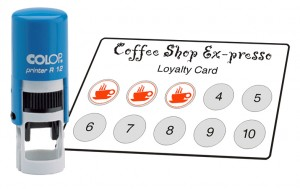
\includegraphics[width=0.5\textwidth]{img/Loyalty-card.jpg}
    \qquad
    
\includegraphics[width=0.3\textwidth]{img/smartcard.png}
    \caption{A paper stamp card \& smart card}%
    \label{fig:smartcard}
\end{figure}
\clearpage{}

\section{Rationale}
The smartphone is now a staple item which many people cannot leave their home without. As of 2014, there is a worldwide user-base of approximately 1.75 billion smartphone devices~\cite{smartUsers}. Migration to phones allow the business to have a central hub of all of their loyalty schemes, eradicating the need for paper. This means that issues relating to paper-based systems, such as printing paper (environmental impact) and people losing their stampcards are no longer an issue. Moreover, businesses will now have the option to track use and monitor their schemes for further analysis. This grants them insight into how users participate in their schemes, allowing businesses to adjust loyalty schemes appropriately.

On the other hand the proposed solution is not without some problems of its own. For instance, not everybody owns a smartphone, so hybrid smartphone/paper solutions will need to be considered. Additionally, there are specific disadvantages of smartphones, such as dependence on battery life and an internet connection.

\section{Aim}
The aim of this project is to develop a general purpose solution using a smartphone that supports businesses in creating, managing and deploying a simple loyalty scheme - using gamification elements to engage the users. The specific technology chosen is NFC in phones running the Android operating system. 

\section{Objectives}
\label{sec:objectives}
\begin{itemize}
    \item Research the state-of-art surrounding NFC technology within loyalty and gamification systems
    \item Examine and analyse the current smartphone solutions available to manage loyalty systems
    \item Design and implement our solution
    \item Perform a field study with the system as an evaluation
    \item Look into the future possibilities of the system and the infrastructural requirements to support its use in a real-world environment
\end{itemize}

\section{Deliverables}
The primary deliverables we perceive for this project are two Android applications. A `Loyalty Stampbook' application for consumers to collect, manage and use their loyalty schemes -- along with a `Loyalty Manager' for businesses/employees to distribute `stamps' to customers via NFC.  

\section{Significance \& Contributions}
NFC is a topic rising in popularity. Many new mobile smartphones now have a chip for NFC communication and many businesses are moving their `card' based services onto smartphones. As such, it is beneficial to explore the possibilities of transferring traditional loyalty cards into the digital era. 

Our solution provides a unique paper-less way for businesses to deploy a loyalty scheme. We attempt to alleviate much of the hassle and cost to businesses with regards to implementation.

Moreover, we aimed to keep the solution very generic as to allow an element of branding and customisability, as well as using open protocols to extend the system to other mobile operating systems.   

\subsection{Similar Developments}
There exist some similar mobile-based solutions to the one proposed, such as Apple's \emph{PassBook}. Passbook is an iOS exclusive application that allows users to save their generic cards (i.e. boarding passes, event tickets, loyalty cards etc.) Though also a general purpose solution, there is a distinction on the technologies used (QR/Barcode Scanning) and the interactions presented to the users - For example, Passbook entails the one-way interaction of simply scanning barcodes. By adopting the two-way possibilities provided by NFC, richer interactions can be built and allow inter-communication between devices. Section \ref{sec:NFCvsQR} will discuss the advantages and disadvantages of each technology.

Other loyalty applications also exist, some using some combination of NFC or gamification elements; nonetheless they are specific to their associated brand. Starbucks' application on iOS is one such example (Fig.~\ref{fig:starbucksios6}), offering users a digital QR version of their Starbucks card (Fig.~\ref{fig:starbucksios6}c) and a medium to collect rewards in the form of stars. These stars, along with the account balance can be used to claim rewards and beverages.

\begin{figure}[h!]
  \centering
    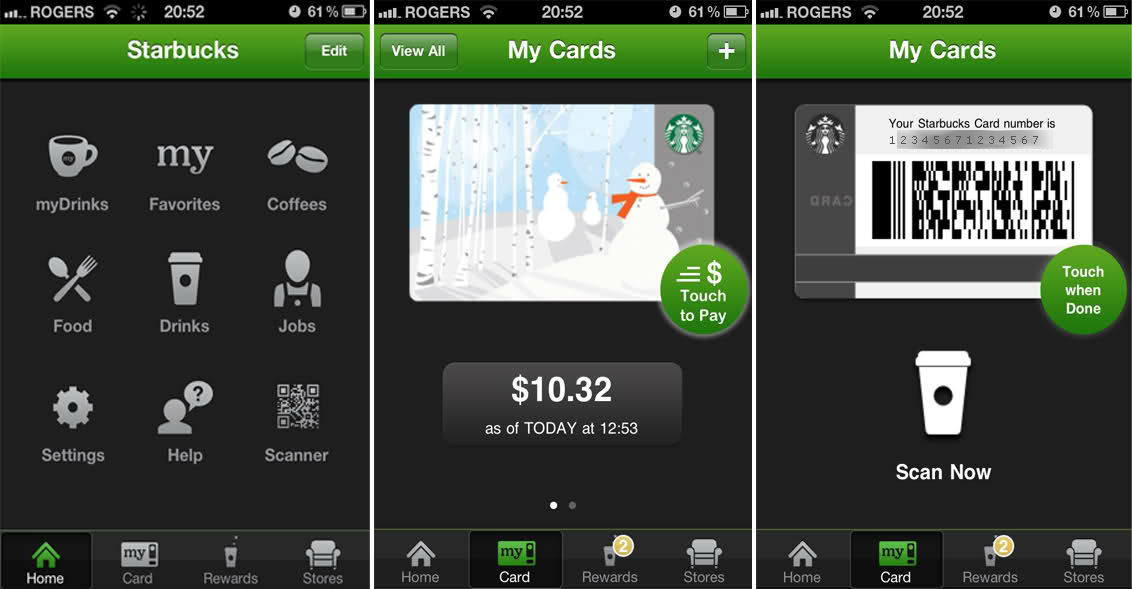
\includegraphics[width=1\textwidth]{img/starbucks-image-2.jpeg}
      \caption{Starbucks application for iOS6 (a) The menu of the Starbucks app (b) The card and available balance (c) The bar-code presented to the baristas to scan}
      \label{fig:starbucksios6}
\end{figure}

In the literature survey we shall cover primary technologies and research that enable these developments, along with confirming the need for a general-purpose solution.

\section{Resources Required}
\subsection{Technologies}
\subsubsection{Android Platform}
Android is a smartphone operating system developed by Google. Along with Windows Mobile OS and Apple's iOS, these three operating systems are the biggest players in the global smartphone market. Android was selected for our system was most devices are equipped with an NFC chip and have well supported APIs regarding Host Card Emulation (See \ref{sec:initalHCE}). With the introduction of iOS8, Apple added support for NFC payments that work with the new iPhone 6; however APIs are unavailable to developers at this time and as a result, cannot be used. Windows Phone has similar NFC libraries to Android, but was not chosen due to it's low market share (2.5\% as a pose to Android's 84.7\%)\cite{marketShare}. 
\subsubsection{Android SDK}
The Android Software Development Kit (SDK) Will be required to develop, implement and test the Android applications. There are several methods that can be chosen regarding Android application development without having to use Google's JAVA SDK. Unfortunately, due to the specific dependencies on Google's NFC APIs, development will need to be done using the JAVA SDK.
\subsubsection{Host Card Emulation (HCE)}
\label{sec:initalHCE}
NFC chips can be placed into Card Emulation mode in such a way (ISO 14443) that a contactless reader classifies it in the same manner as a smartcard.\cite{ecosystem}. Implementation of the system is dependent on use of this NFC facet. \emph{Android 4.4 Kitkat} and above support this mode within the APIs.
\subsection{Android Devices}
For most cases of Android development, the bundled emulator with Google's Android SDK is sufficient; however due to the project's dependence on the NFC chip, at least two physical (preferably differently branded) devices need to be used. One will be running the Loyalty Manager, whilst others will be running our Loyalty Stampbook. Both devices must at least have the \emph{Kitkat 4.4} iteration of Android in order to use Host Card Emulation.

\section{Dissertation Overview}
The rest of the dissertation is presented in the following chapters:
\begin{description}[leftmargin=!,labelwidth=\widthof{\bfseries Medium}]
    \item[Chapter 2] \emph{Literature \& Technical Survey} -- Here we will introduce the research topics of `NFC', `gamification' and `persuasive technologies' and review their applications to the world of mobile applications. 
    \item[Chapter 3] \emph{Requirements \& Design} --- Divulges the process of outlining the design of the system.
    \item[Chapter 4] \emph{Implementation} --- A detail account of the system was built, along with the novel challenges presented. 
    \item[Chapter 5] \emph{Evaluation} --- A field study with users in a natural environment. We attempt to gather quantitative and qualitative feedback, whilst trying to quantify the impact of gamification within the system. 
    \item[Chapter 6] \emph{Discussion} --- We present the results from our study, explaining the areas in which it was successful and what improvements will need to be made. 
    \item[Chapter 7] \emph{Conclusions \& Future Work} -- A closing discussion for our system and the vision for the future. 
\end{description}

\chapter{Literature \& Technical Survey}
\section{Introduction}
This chapter will explore the state-of-the-art surrounding near field communication, gamification and persuasive technologies, along with some current solutions implemented by the industry.

It is anticipated that the main deliverable for this dissertation would be two Android mobile applications to facilitate the creation, deployment and management of a Loyalty Scheme. As such, we will need to discuss the pressing research, benefits and issues that encompass creation of `sticky' technologies on mobile platforms. 

\section{Near Field Communication (NFC)}
Near Field Communication (NFC) is an up-and-coming wireless technology that is currently being adopted in many contexts. Using this proximity-based standard, Two individuals can share data by placing NFC-enabled devices within a few inches of eachother.(see example in Figure 1.1). The standard was first established by Nokia, Philips and Sony in 2004 to define next generation radio frequency communications~\cite{nfcforum}.
\begin{figure}[H]
  \centering
    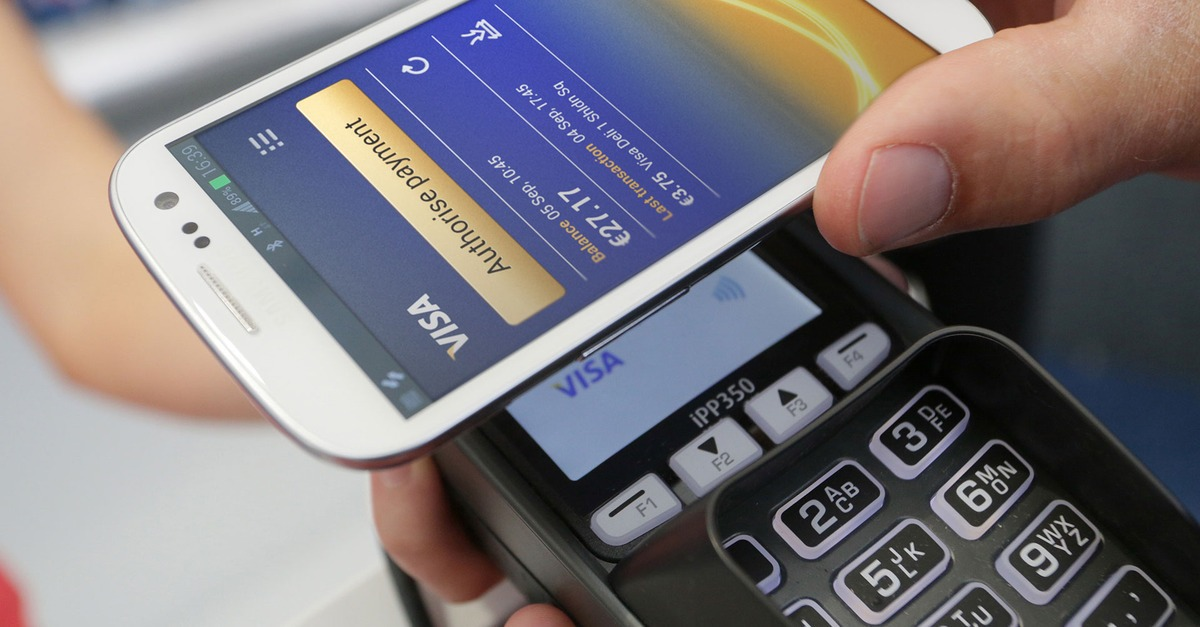
\includegraphics[width=1\textwidth]{img/visa-nfc-samsung.jpg}
      \caption{Using the smartphones NFC chip with a VISA application on a wireless card reader as a form of contactless payment}
\end{figure}

\subsection{Technical Fidelity of NFC}
NFC is a close relative to Radio Frequency Identification (RFID), using the 13.56 MHz radio frequencies under 424Kbit/s bandwidth~\cite{nfcloyal}; however it operates at a far shorter range (10cm versus 100m). As with RFID, there are two types of NFC devices - powered and unpowered. Powered devices surround themselves with an ultra-low power electrical field, inducing electric potential to other NFC devices within range; whereas unpowered devices (also known as ``tags''), rely on this electric potential from powered devices as a power source during the interaction.

NFC devices can adopt several different modes for different interactions~\cite{ventata}

\paragraph{Tag Reading/Writing}
A powered NFC device in this mode can read and write information stored in tags. Websites,  contacts and telephone numbers are commonly encoded in this manner. Upon reading the tag, it is the software's responsibility to act on the data in an appropriate manner~\cite{ecosystem}

\paragraph{Host Card Emulation}
NFC chips can be placed into Card Emulation mode in such a way (ISO 14443)~\cite{iso14443} that a card reader classifies it in the same manner as a smartcard. NFC devices can keep different cards in storage and switch between emulating them as required.~\cite{ecosystem}

\paragraph{Peer-to-Peer}
Two powered NFC devices can bidirectionally share information between each other - for instance Bluetooth pairing information.~\cite{ecosystem}. In the case of a business environment, authentication can take place between two devices in the same bidirectional manner~\cite{iso18092} as a form of `secure log-in'.

\clearpage{}
\subsection{Applications of NFC}
Wireless communication technologies such as NFC have been around for some time. Many electrical devices with the capacity to communicate already use Wi-Fi, Infrared or Bluetooth; eventually these technologies make their way into modern smartphones and other domestic devices. Due to the openness of the NFC standard, there are a wide plethora of implementations facilitated by the technology:
\paragraph{\textbullet~Contactless Payment/Mobile Wallet}
Starting from 2005, banks began integrating contactless chips inside debit/cards for payments under 20 USD/GBP (provided that the card reader supported contactless). From 2011, several large players such as Google, Apple and Paypal have developed mobile wallet applications, with Google and Apple primarily supporting NFC. Contactless cards too rely on the (ISO 14443)~\cite{iso14443} smartcard standard, complementing the previously discussed host card emulation, allowing an NFC chip to emulate an identical smartcard. Whereas, contactless debit and credit cards are prevalent, Google Wallet and Apple Pay are not available outside of the US Market, reasonings being ill-documented.
\paragraph{\textbullet~Ticketing}
Contactless ticketing has been available for a while, the Oyster card\cite{oystercosts} being an iconic example; nonetheless it has the issue of being a proprietary, locked down technology. In 2014, contactless cards were enabled within the system. Some argue that the goal of removing cash-payments was a driving factor of the acceptance of contactless ticketing~\cite{oystercosts}. Moreover, Host Card Emulation infers that mobile wallet applications would also be able to take advantage of these readers.
\paragraph{\textbullet~Gaming}
Game designers have always looked for ways to make video games more engaging. There are two methods in which they can implement NFC within their games, with the intent to make \textbf{Pervasive Games}. Such games expanding the play space into the player's ordinary social life~\cite{montola2005exploring}. Firstly, they may may use NFC to enrich collaboration and sociability. As an example, a study was done with two identical games, one with NFC and the other without\cite{wolbert2013evaluating}. Experiments were ran with two groups of individuals and findings showed a sharp increase in positive experience for NFC over touchscreen~\cite{wolbert2013evaluating} 

The second and more recent way NFC can be implemented in video games is through physical-digital mappings. The \emph{Wii U}~\cite{nintendo} video game console contains an NFC chip in the controller, allowing users to use NFC enabled figurines on the controller. The result of tapping these devices together makes figurines appear within the console as in-game characters. 

\paragraph{\textbullet~Loyalty Schemes}
Loyalty using NFC is a topic that is still being explored by industry. As such, there are some different and creative implementations available. The original NFC Loyalty solutions came in the form of staff/store cards; however with the advent of NFC in mobile phones, pervasive solutions have been implemented such as \emph{Orange EAT}~\cite{orangeEat}.  In this scheme, consumers can tap specific NFC posters and tags in order to gain free rewards in the form of food and drink~\cite{orange}. Unfortuantely this promotion was unsuccessful as at the time only 200,000 customers had an NFC enabled device on Orange (less than 1\% of the total customer base)~\cite{orange}. There are several other prototype solutions available; nonetheless they were not properly adopted as NFC was not available on enough phones.
\clearpage{}
\subsection{NFC in Phones}
NFC functionality in phones is actually not a new concept; phones with NFC chips have been around since 2006, but the adoption of NFC with manufacturers did not get popular until 2010 when a set of peer-peer standards were released to transfer useful information (contacts, URLs and bluetooth)~\cite{iso18092}. Since then, popularity took off, with IHS\footnote{IHS inc is a data and critical information provider for the technology industry} predicting that 939 million NFC enabled handsets would be shipped in 2018 (Fig. \ref{fig:smartphoneshipments})~\cite{IHSchart}.
\begin{figure}[H]
  \centering
    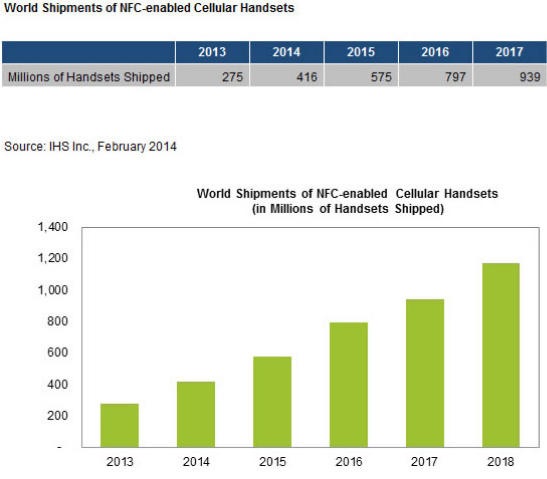
\includegraphics[width=0.8\textwidth]{img/smartphoneNFC.png}
      \caption{A chart depicting the predictions of mobile phones shipments that have NFC built-in}
       \label{fig:smartphoneshipments}
\end{figure}

Interestingly, of all the applications mentioned in the above section, \textbf{all} of them have been implemented both with and without mobile phones. The advantage of using the mobile phone is that it has the capability to consolidate a potentially infinite amount of NFC cards, tags etc into just one chip.

Software support for NFC is something that must be accompanied with hardware. Android and Symbian implemented software support in 2011, Microsoft in 2012 and Apple in 2014. The fact that these implementations are very recent can be attributed to the rising popularity of NFC. 

\subsection{Areas of Research}
In 2010 a survey was done of academic papers surrounding NFC \cite{nfctable}. The authors gathered a total of 74 research papers and used content-oriented classification~\cite{ngai2008rfid} in order to split up NFC papers into four categories: NFC Theory, NFC Applications, NFC Infrastructure and NFC Ecosystem. The results of their findings are shown in table \ref{table:nfcresearch}.
\begin{table}[H]
\resizebox{\textwidth}{!}} \\ \midrule
\multicolumn{1}{|l|}{\begin{tabular}[c]{@{}l@{}}\textbf{NFC Applications and Services}\\ Reader-Writer Mode Applications\\ Host Card Emulation Applications\\ Peer-to-Peer Applications\end{tabular}} & \multicolumn{1}{l|}{Discussing or developing different implementations of NFC applications and services based of NFC modes} & \multicolumn{1}{c|}{30} & \multicolumn{1}{c|}{\begin{tabular}[c]{@{}c@{}}\textbf{40.5}\%\\ 25.7\%\\ 13.5\%\\ 1.35\%\end{tabular}} \\ \midrule
\multicolumn{1}{|l|}{\textbf{NFC Infrastructure}} & \multicolumn{1}{l|}{Types of NFC technologies and their applications in the real world, also security and privacy} & \multicolumn{1}{c|}{22} & \multicolumn{1}{c|}{\textbf{29.7\%}} \\ \midrule
\multicolumn{1}{|l|}{\textbf{NFC Ecosystem}} & \multicolumn{1}{l|}{frameworks for businesses that want to integrate NFC culture \& models and strategies into their processes} & \multicolumn{1}{c|}{7} & \multicolumn{1}{c|}{\textbf{9.5\%}} \\ \bottomrule
\end{tabular}
}
\caption{Table showing the primary categories of NFC research}
\label{table:nfcresearch}
\end{table}

It can be observed that a huge proportion of NFC literature (40\%) at the time was heavily focused on developing prototype applications and services. However, the specific types of applications were primarily `Reader-Writer' mode as this was just before the introduction of NFC peer-to-peer standards.

The research identified that there was a gap in researching the development of NFC principles and theories or how to integrate such solutions into business models. As a result, we can argue that this business-orientated business gap was a factor for the slow adoption of NFC.
\subsection{Limitations of NFC}
The key limiting factor of NFC for the longest time was the slow adoption rate by businesses and manufacturers. Contactless payment, the predominate form of NFC interaction depended on specific NFC card readers to enable contactless functionality; furthermore we cannot underestimate the amount of effort it takes to introduce a new billing option to a country.

Analytics also show that NFC implementations are very fragmented with no apparent standard protocols~\cite{fragmentednfc}. This can be attributed to two reasons: the openness of the NFC platform encouraging different implementations and businesses wanting their own implementation for their own needs. For instance, in the example of loyalty schemes, each business might have a separate loyalty application which the customer needs to download and setup. These applications allow businesses to perform their own tracking and branding.
\newpage
\subsection{NFC vs Quick Reference Barcodes}
\label{sec:NFCvsQR}
Another technology considered for communication was \emph{Quick Reference (QR) Barcodes} (Fig. \ref{fig:qrcode}). These convey information through a 2D code matrix which can be scanned by a barcode reader or optical camera. A summary follows of the advantages and disadvantages of each technology~\cite{nfcadv}\cite{qradv}:

\begin{figure}[H]
  \centering
    
\includegraphics[width=0.15\textwidth]{img/qrcode.png}
      \caption{An example of a QR code}
       \label{fig:qrcode}
\end{figure}


\subsubsection{Analysis of QR}
The advantages (+) and disadvantages (-) of QR are: 
\begin{description}[leftmargin=!,labelwidth=\widthof{\bfseries small}]
	\item[+] QR Codes can be cheaply printed on paper. No tags need to be involved.
	\item[+] Smartphones need only a camera and QR Reader application to interact with the technology
	\item[+] They are generally seen as more secure as they exist outside of a mobile operating system, making them less vulnerable to exploitations.  
	\item[---] Reading a QR code is a much slower interaction as it requires an actor to have a camera app open to scan the barcode. 
	\item[---] QR code scanning is generally seen as one-way interactions as barcode readers have no way to communicate with the barcode (physical/digital).
	\item[---] QR codes cannot hold dynamic information. In order to change the sent message, a new barcode will have to be generated
\end{description}

\newpage
\subsubsection{Analysis of NFC}
The advantages (+) and disadvantages (-) of NFC are: 
\begin{description}[leftmargin=!,labelwidth=\widthof{\bfseries small}]
    \item[+] NFC Interactions are much simpler and faster as they only involve a tap
    \item[+] NFC chips can dynamically change their contents without having to generate a new tag/device
    \item[+] NFC affords compatibility with many standard smartcard readers
    \item[+] Two-way interactions are possible, where both NFC chips can communicate with each other in duplex. 
    \item[---] Requires NFC enabled smartphone in order to operate
    \item[---] cannot simply be `printed out on paper' -- an NFC tag must be purchased
    \item[---] very short range of NFC makes it difficult to eavesdrop on; nonetheless it is still possible
\end{description}

\subsubsection{Research}
Many researchers~\cite{qr1}\cite{qr2}\cite{nfc1}\cite{nfc2} provide conflicting opinions regarding which of these technologies should be mass adopted. As NFC chips have taken a substantial amount of time to be integrated into modern smartphones, QR codes were embraced by many businesses as many smartphones can display/read them. On the other hand, the commonality of NFC in modern smartphones narrows this gap in availability. Some solutions have chosen to overcome this gap by creating hybrid systems that support both technologies~\cite{NFCandQR}

\subsubsection{Justification for NFC}
For our system, speed over availability is needed as we want the interaction to be at least as fast as stamping a paper card. A system like this cannot afford to complicate such a simple interaction; therefore we confirm the viability of NFC as our chosen communication technology. 

%%%%%%%%%%%%%%%%%%%%%%%%%%%%%%%%%%%%%%%%%%%%%%%%%%%%%%%%%%%%%%%%%%%%%%%%%%%%%%%%%%%%%%%%%%%
%                                 GAMIFICATION SECTION
%%%%%%%%%%%%%%%%%%%%%%%%%%%%%%%%%%%%%%%%%%%%%%%%%%%%%%%%%%%%%%%%%%%%%%%%%%%%%%%%%%%%%%%%%%%
%About 20 percent of phones worldwide might have NFC capabilities by 2014 [source: Juniper].
\clearpage{}
\section{Gamification}
Over the years, a keen topic of research within Human Computer Interaction is that of user engagement. There are several different design models that afford this goal. One recent and popular example being gamification. 

Gamification can be best described as
\begin{quotation}
\noindent
``An informal umbrella term for the use of video game elements in non-gaming systems to improve user experience (UX) and user engagement.''~\cite[p.~2425]{Deterding:2011:GUG:1979742.1979575}
 \end{quotation}

%talk about user engagement stuff/ studies
The need for gamification comes from the modern zeitgeist of the digital world, a world of engagement. Comparing the current opportunities for entertainment (i.e. video games, social media, the internet) to those from fifty years ago, provide users with much more choice. Furthermore, users are no longer registering traditional advertising in the same way they did fifty years ago. A study done with university students using eye-tracking technology with \emph{Facebook} shows that students perceive less than a quarter of the site's adverts~\cite{barreto2013users}. Experimenters concluded that this was due to users scrolling the timeline too quickly and learning where advertisements appear, therefore ignoring those areas. 

By harnessing the power of play, designers can apply motivational affordances to improve user engagement. Gamification techniques are predicted as the future of marketing~\cite{ventata}, with Gartner\footnote{Gartner is an IT research and advisory business} stating that 50\% of companies with innovation processes will incorporate gamification by 2015~\cite{gartner50}.

\subsection{History}
The principles of ``turning things into games'' are actually not new. They have long been employed by parents and teachers to make activities seem more enticing to children; however applying game-like aspects to a business environment was only formally introduced in the 80's~\cite{coonradt1985game}. The word \emph{Gamification} was coined in 2002 by Nick Pelling, an early computer games programmer that wanted to apply game-mechanics to different contexts~\cite{marczewskigamification}. Recently, gamification has become a buzzword amongst modern system designers. The rise in popularity can be shown in a Google Trends search (Fig. \ref{fig:gamificationpopularity}). This boom can be attributed to soaring video game popularity and cheap enabling technologies found in modern domestic appliances (i.e GPS, Internet Access, Bluetooth etc.)~\cite{Deterding:2012:GDM:2212877.2212883}

\begin{figure}[H]
  \centering
    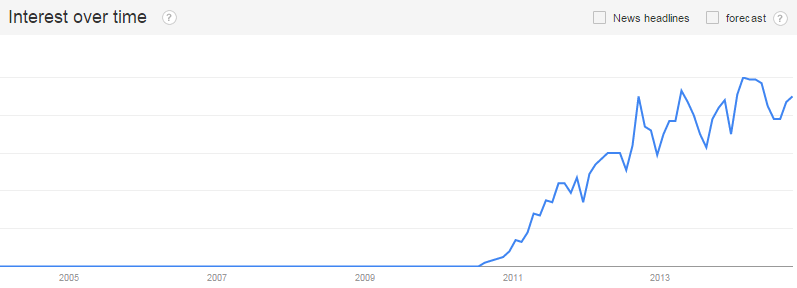
\includegraphics[width=1\textwidth]{img/gamification.png}
      \caption{Google Trends graph depicting the search popularity of the term \textbf{Gamification} over the years}
      \label{fig:gamificationpopularity}
\end{figure}


The use of gamification has also shifted over the years. Many reseachers~\cite{deterding2014ambiguity}\cite{park2014study} consider Charles Coonradt as pioneer in the field of gamification. In his acclaimed book \emph{The Game Of Work}~\cite{coonradt1985game}, Coonradt introduces ``game-like concepts'' inspired from sports as a means to increase employee productivity, satisfaction and motivation~\cite{coonradt1985game}. On the other hand, gamification in the digital age takes inspiration from video games to to improve user experience, engagement and loyalty.~\cite{ventata}

It can be argued that the two inspirations (sports vs. video games) present us with different flavours of gamification. Games of sport entail clear goals, instantaneous feedback, and the concept of striving to be better. Video games aim to keep players playing by providing psychological rewards such as achievements, unlocks and ability to compare their skill with their friends. Even though these two methods of gamification have some differences, their main shared trait lies in the way they play on our natural instinct of socialisation and competition. ~\cite{grove2011gamification}

\subsection{Gamification and Mobile Technologies}
Although elements of gamification can be found in a variety of systems, mobile technologies have seen biggest boom in gamified systems. As mentioned earlier, a major contributer to this boom is the prevalence of cheap enabling technologies such as bluetooth, and GPS - all of which can be found on a modern smartphone. In 2009, Foursquare was one of the first successful gamified mobile applications; allowing users to ``check-in'', collect badges and receive recommendations on where to go next~\cite{zichermann2011gamification}. Five years later, Gartner predict that 70\% of the top 2000 companies would have a gamified application by the end of 2014.~\cite{gartner70}

\subsection{Areas of Research}
A survey was done of academic papers in 2014 analysing gamification~\cite{gamificationlit}. 24 Papers were gathered that involved empirical studies to answer the question `does gamification work?'. Papers were broken down by gamification elements (shown in Table \ref{tab:game1}) and system purpose (shown in Table \ref{tab:game2})

\begin{table}[h]
\begin{tabular}{@{}ll@{}}
\toprule
\textbf{\begin{tabular}[c]{@{}l@{}}Motivational\\ Affordance\end{tabular}} & \textbf{Papers Containing} \\ \midrule
Points & 9 \\
Leaderboards & 10 \\
\begin{tabular}[c]{@{}l@{}}Acheivements/\\ Badges\end{tabular} & 9 \\
Levels & 6 \\
Story & 6 \\
Theme & 4 \\
Clear Goals & 6 \\
Feedback & 6 \\
Rewards & 4 \\
Progress & 4 \\
Challenge & 7 \\ \bottomrule
\end{tabular}
\caption{Table containing the how many papers referenced certain gamification techniques}
\label{tab:game1}
\end{table}

It is easity identifable that points, leaderboards and badges are the most commonly implemented techniques. This can be attributed to social media, as these three affordances are ideal for competition between friends. Interestingly, not very many papers referenced rewards, which may not be as strong of a motivator as competition.

\begin{table}[h]
\begin{tabular}{@{}ll@{}}
\toprule
\textbf{Application} & \textbf{Papers} \\ \midrule
Commerce &  1\\
Education & 9 \\ 
Health & 1 \\
Organisational & 4 \\
Sharing & 1 \\
\begin{tabular}[c]{@{}l@{}}Sustainable\\ Consumption\end{tabular} & 1 \\
Work & 4 \\
Innovation \& Ideation & 2 \\
Data Gathering & 1 \\ \bottomrule
\end{tabular}
\caption{Research papers broken down by system purpose of analysed implementations}
\label{tab:game2}
\end{table}

True to the roots of gamification, many analysed systems were used in an educational manner. On the other hand, many other applications seem to be vastly unexplored, including commerce and work which are the contexts of our system -- hinting a gap in the market gamification for those areas. 

\subsection{Critiques of Gamification}
The application of gamification practises to digital applications is prevalent amongst business applications~\cite{gartner70}, nonetheless these practises have attracted criticisms. One view adopted by the video games industry is that gamification mistakenly portrays ``game-like'' properties, such as levels and scores as part of human behavioural complexity.~\cite{bogost2011gamification}. Moreover, there are negative ``exploitative'' connotations (discussed later) to word gamification in the business world; therefore businesses generally prefer the term ``motivational design'' instead. 

The concept of creating ``sticky'' systems via gamification techniques can also present us with systems that affect user behaviour negatively. The McDonalds Monopoly sweep-stake is a well known example of this phenomenon. The promotion involves the collection of monopoly stickers containing prizes from purchasing certain food and drink (more stickers with larger meals). Paxman et al~\cite{mcdonalds} introduce examples where consumers change their purchasing habits in order to maximise the number of stickers they receive, linking these changes to childhood obesity~\cite{mcdonalds}. Several theories of motivation exist explaining these behaviours; however Zichermann~\cite{zichermann2011gamification} considers motivational factors as unruly, yet admits ``once you start giving someone a reward, you have to keep [them] in that reward loop forever''~\cite[p.~27]{zichermann2011gamification}.

%%%%%%%%%%%%%%%%%%%%%%%%%%%%%%%%%%%%%%%%%%%%%%%%%%%%%%%%%%%%%%%%%%%%%%%%%%%%%%%%%%%%%%%%%%%
%                                PURSUASIVE SYSTEMS                                       %
%%%%%%%%%%%%%%%%%%%%%%%%%%%%%%%%%%%%%%%%%%%%%%%%%%%%%%%%%%%%%%%%%%%%%%%%%%%%%%%%%%%%%%%%%%%
\section{Persuasive Technologies/Captology}
Capturing the attention of an person for the purposes of persuading them is a problem that sympathises with many. Businessmen, politicians and teachers alike are examples of such professions - more specifically professions where persuasion is an integral factor of their success. There exist a plethora of methods to achieve this, for instance salesman study marketing, politicians study public speaking, whilst those in the realm of technology study captology (the art of persuasive technologies).

We can define `persuasive technologies' as:
\begin{quotation}
\noindent
Solutions which are designed with a purpose to change attitudes or behaviours via persuasion and social influence, but not through coercion~\cite{fogg}[p.10]
\end{quotation}

Fogg, considered by many~\cite{fogg1}\cite{fogg2} as a pioneer in the research of captology, identifies the art as an intersection between technology and persuasion (Fig. \ref{fig:captologyVenn}). 

\begin{figure}[H]
  \centering
    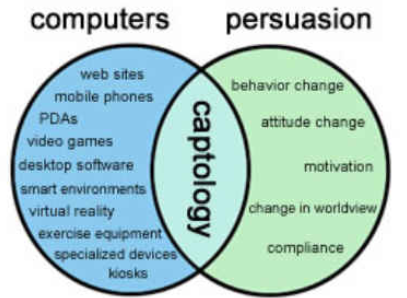
\includegraphics[width=0.5\textwidth]{img/captology-figure-3.png}
      \caption{A Venn diagram showing the intersection of persuasion and technology - Captology}
      \label{fig:captologyVenn}
\end{figure}

\subsection{Types Of Motivation}
It is also helpful to mention the types of motivations which affect people to do activities. Literature indicate that there are three main types of motivators that drive people to behave in a certain way, Deci and Ryan~\cite{motivationtypes} define them as:
\begin{quotation}
\noindent
\textbf{Extrinsic Motivation}~ Incentives where motives to enact the task are not related necessarily to that specific behaviour - \textit{i.e. Completionism}

Extrinsic motivation takes the form of leveraging the human Psyche. For instance, the example of a progress bar persuades the user to bring it up to 100\%. The user may not be specifically motivated to perform the task, but they are motivated to complete the progress bar.
\end{quotation}
\begin{quotation}
\noindent
\textbf{Intrinsic Motivation}~ The act of making the intended behaviour so pleasurable that it becomes an end in itself - \textit{i.e. Gamification}

The philosophy of this motivator is to persuade the user to engage with the activity in a way that they enjoy. Gamification exists within this realm of motivation, making activities more enticing to users.
\end{quotation}
\begin{quotation}
\noindent
\textbf{Tangible Motivation}~ External Incentives driving the motivations - \textit{i.e.Rewards/Money}

These motivators usually offer some sort of reward such as money to entice the user to perform an action. Although only considered as short-term, it is useful at incentivising one-off activities that are difficult to make engaging, for example surveys. 
\end{quotation}

Persuasive technologies afford the use of any combination of these to develop systems. We discuss an example in Sec. \ref{sec:piano}

\subsection{Fogg's Taxonomy}
Fogg characterises each persuasive technology by \emph{functional roles}: tools, media or social actors.~\cite{fogg1998persuasive}, of which technologies can identify as one or several of these categories. The proposed triad is designed to model the way in which users see and react to the following:

\paragraph{Tools}
These technologies are designed to make people's jobs easier\cite{fogg}. For example a wizard or an Out of Box Experience (OOBE) can give users direction regarding the completion of a specific or complex user task.
\paragraph{Media}
Media-centric technologies are designed to provide users a platform to create experiences that develop, teach or enforce a behaviour. These can come in the form of games, interactive systems or stories;  the best examples however are simulations. Simulations place the users in a specific environment where they must interact with rules of the system in order to hone a required set of behaviours; such behaviours can be for the purposes of testing or real-life skills. 
\paragraph{Social Actors}
With the introduction of social actors, computer systems can now influence users using social cues. Actors can be persuasive by giving a human face to positive feedback, modeling an inded behavior or provide moral support to the user~\cite{fogg}. The \emph{Microsoft Paperclip} is a famous example of a social actor to teach users how to use Microsoft Office. Research in this area is constantly developing as it's difficult to build `human' characters without entering ``uncanny valley''.
 
%A social actor can be persuasive byreddit.com
% Rewarding people with positive
%feedback
% Modeling a target behavior or
%attitude
% Providing social support

\subsection{Persuasive Technologies Through Gamification}
\label{sec:piano}
Persuasive Technology is a broad term. As such, it can be argued that gamification exists within the realm of captlogy; nonetheless there exists the key differentiators of scope, more specifically - gamification is not necessarily linked to technology (although `gamified' technologies are generally more common).
%gamification just makes something more enticing , whereas captology

A well known case study of implementing persuasive technologies using gamification are The Piano Stairs (Fig. \ref{ref:pianostaircase})~\cite{tieben2011curiosity}. In this example, tiles and speakers in the configuration of a piano were installed next to an escalator, each stair playing a specific note on the piano when stepped on. The purpose of this experiment was to get more commuters to take the `healthier' stairs rather than the escalator. Results showed that people were taking the stairs frequently and in more `musical ways', with some musicians attempting to play songs using them. There was however another factor that encouraged people to take the stairs: curiosity~\cite{tieben2011curiosity}. The staircase is so out of place that people are curious and thus want to explore and engage with the technology.

\begin{figure}[H]
  \centering
    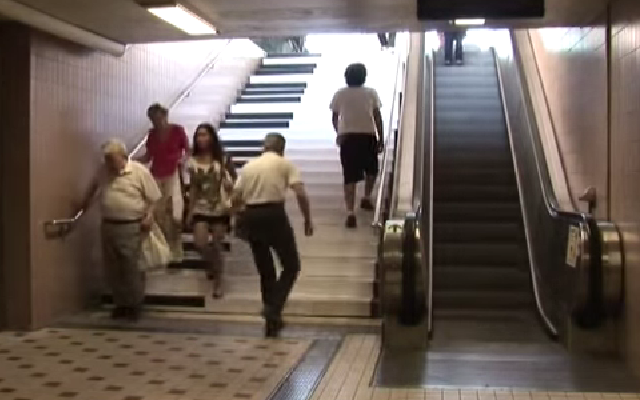
\includegraphics[width=0.7\textwidth]{img/pianotiles.png}
      \caption{The piano tiles staircase}
      \label{ref:pianostaircase}
\end{figure}

Applying the concept of Fogg's taxonomy and motivator types, this innovation is an example of a media-oriented technology, fueled by intrinsic motivation - making the act of going up the stairs more enjoyable. Although empirical evidence on users after taking the stairs was not tracked, it would be interesting to see whether these stairs impacted people's choice of taking other stairs in the long run. 

%%%%%%%%%%%%%%%%%%%%%%%%%%%%%%%%%%%%%%%%%%%%%%%%%%%%%%%%%%%%%%%%%%%%%%%%%%%%%%%%%%%%%%%%%%%
%                                     SOLUTIONS
%%%%%%%%%%%%%%%%%%%%%%%%%%%%%%%%%%%%%%%%%%%%%%%%%%%%%%%%%%%%%%%%%%%%%%%%%%%%%%%%%%%%%%%%%%%
\section{Survey of Technologies}
We now turn our focus to the developed solutions. These technologies were chosen as they use a combination of NFC, gamification or persuasive technologies. The first group will contain implementations dedicated to a certain business; whereas the second will look at more generic applications. The chosen solutions were only those where \textbf{Loyalty} was the core function of the technology, `ecosystem-based' combined solutions were not considered.

In order to summarize these technologies later, each of the following should answer these questions:
\begin{itemize}
  \item How does the user interact between the real world and the applications (what pervasive elements does the application possess)?
  \item What elements of gamification exist?
    \item In what ways are multiple loyalty schemes presented? %levelling up - multiple schemes 
  \item Are there any subtle persuasion techniques employed?
\end{itemize}


\begin{figure}[H]
  \centering
    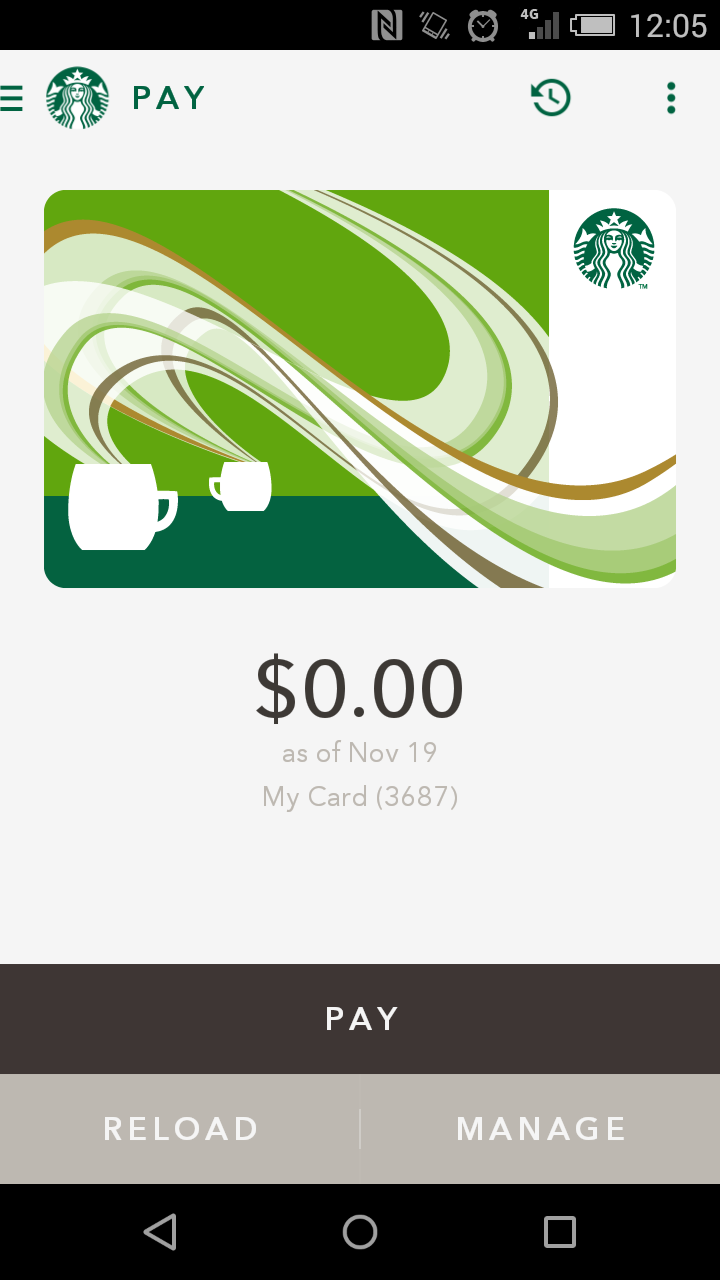
\includegraphics[width=0.24\textwidth]{img/starbucks.png}
    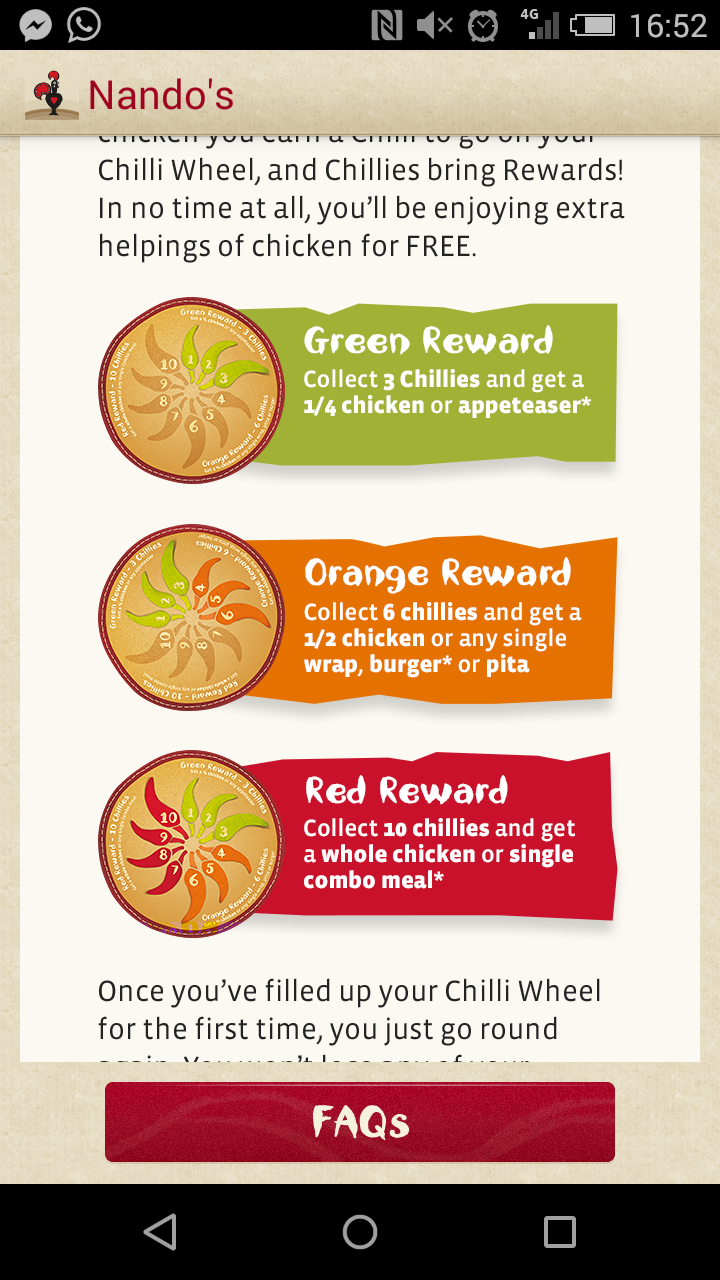
\includegraphics[width=0.24\textwidth]{img/nandos.png}
    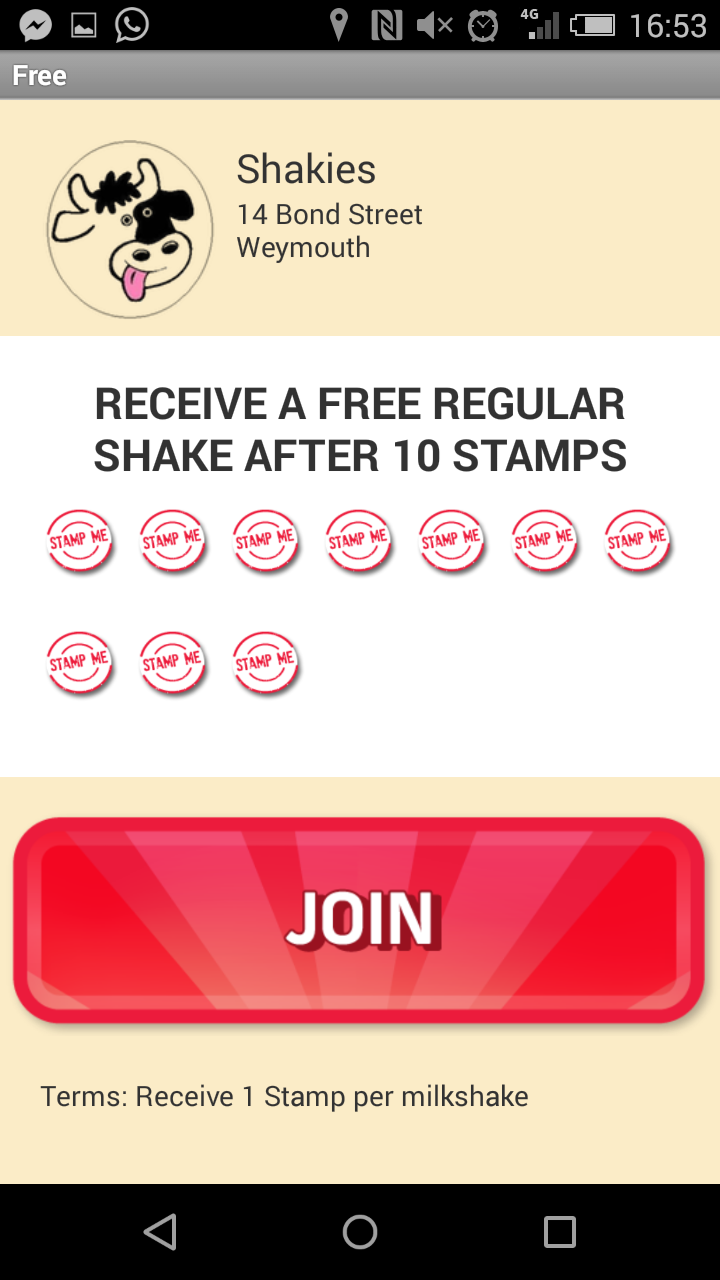
\includegraphics[width=0.24\textwidth]{img/tagmate.png}
    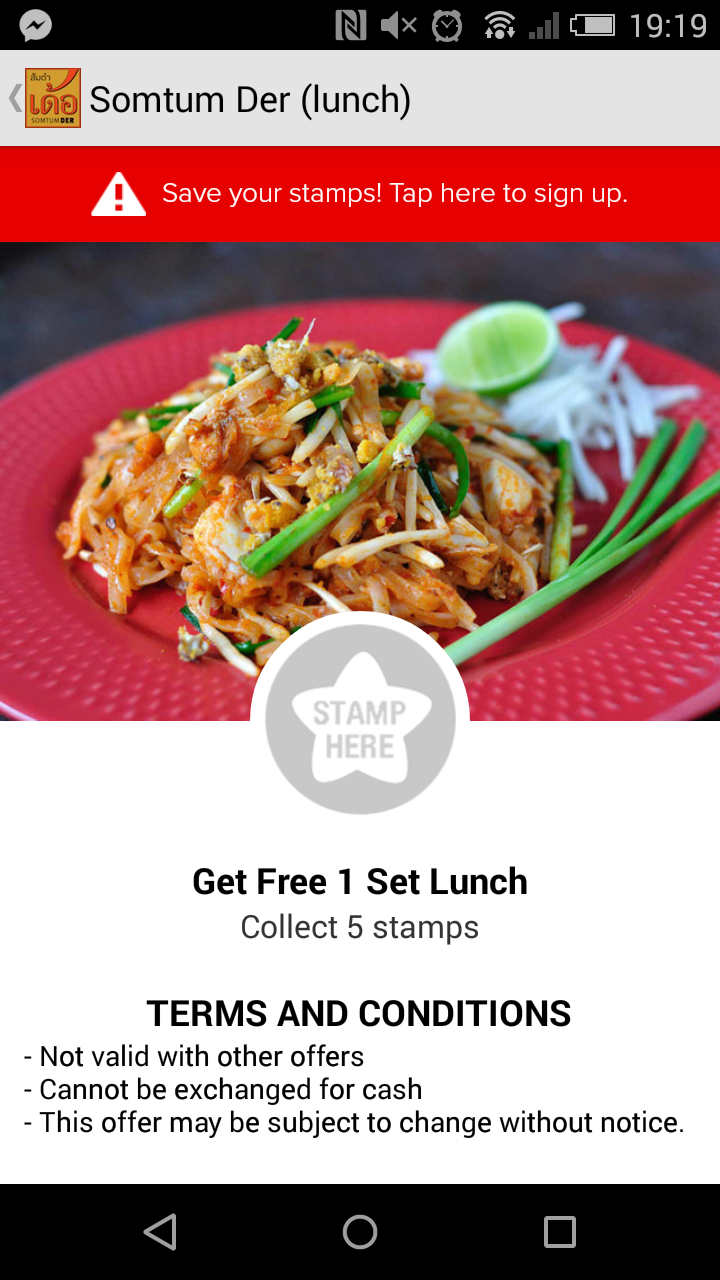
\includegraphics[width=0.24\textwidth]{img/stamp.png}
      \caption{The technologies to be analysed: (a) Starbucks (b) Nandos (c) StampMe (d) Stamp}
\end{figure}

\subsection{Starbucks Mobile Application}
\textbf{Overview}
The Starbucks mobile application is designed as a digital-companion to the standard plastic loyalty card they provide. The application allows user's to either have a digital-only card or transition their physical cards onto the app, allowing customers to view, top up and pay with their balance.

\textbf{What are the pervasive elements?}
Aliased Card Using BQ barcode that is scanned by a barista.

\textbf{What elements of Gamification exist?}
Collect Stars with each purchase, free drink on 15, upgrade to gold member upon collecting 50 stars.


\textbf{In what ways are multiple loyalty schemes presented?}
The user can have up to 10 Starbucks cards but only claim free drinks with their stars.

\textbf{Are there any subtle persuasion techniques employed?}
Extrinsic Motivation of filling a cup, personalise your card.
%personalise card

\subsection{Nandos Mobile Application}
\textbf{Overview}
As with Starbucks, the Nandos' mobile application works in a very similar manner to the starbucks card. It allows users to register their current physical card; however this app is purely as a companion, informing users of the status of their loyalty points in the card.

\textbf{What are the pervasive elements?} There are no pervasive methods. The user must have and use a Nandos Card.

\textbf{What elements of Gamification exist?}
No elements of gamification are used.

\textbf{In what ways are multiple loyalty schemes presented?}
Loyalty schemes are presented as a progressive stampcard. Rewards of increasing value are granted upon reaching certain amounts of chillis

\textbf{Are there any subtle persuasion techniques employed?}
When a users connects their card to the app, A wheel with different colored chillis are displayed. In order to get rewards, users must complete the wheel, displaying the example of extrinsic motivation via completionism - encouraging users to fill the wheel. 
\subsection{StampMe \& Stamp}

\textbf{Overview}
StampMe \& Stamp are both general purpose loyalty application for corporates to implement loyalty schemes. Businesses can only have one loyalty scheme that mainly adopts the ``free x with y stamps'' methodology. Users can browse for nearby shops that have available offers and collect numerous schemes.

\textbf{What are the pervasive elements?}
In order to gather a stamp from these apps, the business uses a proprietary digital stamping device to stamp the screen of the mobile phone, thus transferring a stamp. Although this is an interesting way to stamp the screen, information about the specific technology it uses proved impossible to find. It can however be inferred that this technology is not NFC as it works on both iOS (those with and without NFC chips) and Android.

\textbf{What elements of Gamification exist?}
no offers or gamification elements are implemented within these applications. 

\textbf{In what ways are multiple loyalty schemes presented?}
Once a user `joins' a business' loyalty scheme, it is added to a list of their current loyalty programs. The list is made out of simple text and does not display any information about the progress of the schemes - unless they explicitly click on the name of the business first.

\textbf{Are there any subtle persuasion techniques employed?}
These applications attempt to clone a real Stampcard. This is considered a use of extrinsic motivation where users may not necessarily want to buy a coffee but want to complete their stamp card. 

\subsection{Summary of Solutions}
We summarise the fidelity of the above systems into table \ref{tab:solutions}.

\begin{table}[h]
\resizebox{\textwidth}{!}{%
\begin{tabular}{@{}lllll@{}}
\toprule
 & Pervasive Elements & Gamification Elements & Multiple Schemes & Persuasion Techniques \\ \midrule
\textbf{Starbucks} & QR Code & Collecting Stars & None & Fill up cup with stars for a free drink \\
\textbf{Nandos} & None & None & Can claim different rewards depending on amount of built up chillis & Fill the wheel to increase chilli count \\
\textbf{StampMe \& Stamp} & Proprietary System & None & Add multiple loyalty schemes from participating businesses & Affordance of real stampbook appearance \\ \bottomrule
\end{tabular}
}
\caption{A summary of the solutions discussed}
\label{tab:solutions}
\end{table}

Although there exists some general purpose loyalty solutions, they lack the polish and compared to the business-centric applications. On the other hand, those applications that are business-centric require users to install a mobile application for each loyalty card. Whereas large businesses have the resources to create such highly customised, high-fidelity systems, small businesses have little incentive to invest outside of paper-based solutions, mainly due to large development and implementation costs. As a result, they usually invest in the underused general-purpose solutions.

NFC with social elements is an area vastly untapped by businesses, mainly due to the slow uptake of NFC by the market; moreover it seems like those loyalty systems using the proprietary stamping technology seem to be re-inventing the wheel instead of using the open standard.

\section{Conclusions}
In this chapter we covered the concepts of NFC, gamification and persuasive technology in terms of research and current implementations. By analysing similar systems, we justify the need for our system as an encompassing general-purpose solution that any business, big or small, can use to simply implement a loyalty program and push it out to any users of the application; collecting `stamps' using NFC. All loyalty schemes will be automatically incorporated into a gamification framework provided by the application, providing businesses a gamified loyalty scheme with minimal effort.

The next chapter discusses how we identified the system requirements and the process reaching a complete design for the system.

\chapter{Requirements \& Design}
\section{Introduction}
This chapter describes and outlines the requirements for the proposed software solution. Requirements will set goals for the functionality of the software, whereas the design section allows us to translate these requirements onto paper. Both sections will become useful when testing whether the system is fit-for-purpose.

\section{Requirement Methodology}
In this section, system requirements will be presented. Two sources of requirements were used: firstly using information discovered from the literature survey; and secondly from an interview from a project manager at `Company A'. These requirements are not to be used as an exhaustive list, but are to be used as a benchmark for ensuring the created product is fit-for-purpose.

\subsection{The Interview}
To gather business oriented requirements, an interview was conducted with a project manager, specialising in IT implementations for corporate facilities. several points discussed were integrated into the system as requirements. For instance:

{\fontfamily{ppl}\selectfont
6. What do you think of this solution? (The corporate loyalty app)

For this solution to be feasible and useful, it would need to be:

\begin{itemize}
\item Available for all of our permanent staff to use
\item Easy integration for further sites and users globally
\item Good usability aspects. GSK has 100,000 staff members with a variety of demographics, therefore all users should find it easy to use and better than the existing process
\item The system would need to increment on a daily basis when the staff members enter site (once a day only)
\end{itemize}
}

Informed requirements M2, S3, S4, and C4.

The transcript of the interview can be found in the appendices. 

\clearpage{}

\subsection{Requirements}
Our solution involves the creation of two Android applications, thus the requirements below will be marked whether they are for \textbf{Both} or exclusively for the \textbf{Loyalty Manager}, or \textbf{Loyalty Reader}. Effort will be made to maximise cross-system requirements. We found that there was an abundance of potential system requirements, however not all can be implemented in good time. As such, we present these requirements in MoSCoW Format~\cite{brennan2009guide} (Must Have, Should Have, Could Have, Won't Have) in order to categorise the importance of their delivery.

\subsubsection{Must Have}
\begin{description}[leftmargin=!,labelwidth=\widthof{\bfseries Medium}]
    \item[M1] \textbf{Sign-In \& Registration} \newline
        \textit{The user should be able to sign in with an existing account or register for a new one} \newline
        [Both Systems] | Functional
        
    \item[M2] \textbf{Fast Stamping} \newline
        \textit{Access to the NFC stamping functionality should be available within a single tap from a home page} \newline
        [Both Systems] | Functional
    
    \item[M3] \textbf{NFC Transmission} \newline
        \textit{The system must use NFC for data transmission and Host Card Emulation} \newline
        [Both Systems] | Functional
        
    \item[M4] \textbf{Online Syncing} \newline
        \textit{The system must be able to sync a users 'stampbook' online} \newline
        [Both Systems] | Functional
        
    \item[M5] \textbf{Sync on Interaction} \newline
        \textit{Syncing must take place as soon as there is an interaction that affects the stamp count of a scheme} \newline
        [Both Systems] | Functional
        
    \item[M6] \textbf{Syncing Time} \newline
        \textit{The response time for syncing must be within 5 seconds} \newline
        [Both Systems] | Non-functional  
        
    \item[M7] \textbf{Feedback on Interaction} \newline
        \textit{The system must provide audio/visual feedback whenever a 'stamp' has taken place} \newline
        [Both Systems] | Functional
        
\end{description}

`Must have' requirements are the minimum amount of features to be satisfied for the success of the system. As a result, these are of highest priority. Requirements defining gamification are not listed here as they are not `key' to the system.

\subsubsection{Should Have}
\begin{description}[leftmargin=!,labelwidth=\widthof{\bfseries Medium}]
    \item[S1] \textbf{Consistency} \newline
        \textit{The system should fit within the standards and design language of the Android operating system} \newline
        [Both Systems] | Non-functional
        
    \item[S2] \textbf{Secure Communications} \newline
        \textit{NFC Communications between devices should be encrypted} \newline
        [Both Systems] | Functional

    \item[S3] \textbf{Rewards Browsing} \newline
        \textit{The user should be able to easily browse their rewards available} \newline
        [Loyalty Reader] | Functional
        
    \item[S4] \textbf{Levelling System} \newline
        \textit{Users should be able to level up each of their loyalty schemes independently (20 - gold, 50, platinum)} \newline
        [Loyalty Reader] | Functional
        
    \item[S5] \textbf{Level-Restrictions} \newline
        \textit{Rewards should have a minimum-level required in order to claim} \newline
        [Loyalty Reader] | Functional

    \item[S6] \textbf{Badges} \newline
        \textit{Users should be able to collect badges upon completing certain goals} \newline
        [Loyalty Reader] | Functional
\end{description}

The `should have's' represent features which should be included if the system if time permits. Generally these requirements add a layer of usability and engagement to the system; as such, most of the gamification implementation is defined here.

\subsubsection{Could Have}
\begin{description}[leftmargin=!,labelwidth=\widthof{\bfseries Medium}]
    \item[C1] \textbf{Branding} \newline
        \textit{The system could provide deep customisation options for each scheme} \newline
        [Loyalty Manager] | Functional
        
    \item[C2] \textbf{Personalisation} \newline
        \textit{The system could allow users to customise the appearance of their profile} \newline
        [Loyalty Reader] | Functional
        
    \item[C3] \textbf{Passive Card Emulation} \newline
        \textit{The system could allow passive host card emulation} \newline
        [Loyalty Reader] | Functional
        
    \item[C4] \textbf{Restricted Schemes} \newline
        \textit{The system could allow for account-specific schemes (only authorised users have access to the scheme)} \newline
        [Both Systems] | Functional
        
    \item[C5] \textbf{Internet-Free Stamping} \newline
        \textit{Users could have the ability to gather stamps without being connected to the internet (facilitated by the Manager)} \newline
        [Loyalty Manager] | Functional
        
    \item[C6] \textbf{Multiple Device Support} \newline
        \textit{Users could be able to login and use multiple devices seamlessly} \newline
        [Loyalty Reader] | Functional
        
    \item[C7] \textbf{Transaction History} \newline
        \textit{The system could have a transaction history to allow users to see their recent activity} \newline
        [Loyalty Reader] | Functional
\end{description}

These requirements represent bells-and-whistles requirements. Features in the `could have' are desirable but not a necessity to the project's initial builds. Incorporations of these requirements into future builds of the system would greatly benefit user experience.

\subsubsection{Won't Have}
\begin{description}[leftmargin=!,labelwidth=\widthof{\bfseries Medium}]
    \item[W1] \textbf{Payment Options} \newline
        \textit{The system will not facilitate any form of payment} \newline
        [Both Systems] | Functional  
        
    \item[W2] \textbf{Loyalty Sharing} \newline
        \textit{Users will not be able to transfer stamps between friends/accounts} \newline
        [Loyalty Reader] | Functional 
\end{description}

`Won't have' requirements are simply outside the scope of the project. Their functionality is either not the purpose of the system (W1), or facilitate unwanted features into the ecosystem (W2). 






\clearpage{}
\section{Design}
\subsection{Outline}
Turning our attention to the design, here we present the system, matching the requirements, outlining how they meet the system requirements. Some interesting scenarios have been mentioned in the requirements that leave a wide scope of design challenges. A study is also undertaken that involves participatory design as an extension of the proposed design - in effect, asking potential users to tackle these challenges.


\subsection{The Three Components of the System}
As mentioned earlier, the proposed system involves two separate Android applications. However, in order to meet functional requirements M1, M4, S4, S6, C4 and C6 a database will need to be introduced in order to inter-connect user accounts, along with any relevant data (i.e. loyalty schemes, stamps and badges). Furthermore, a database is also useful from a security and continuity standpoint. For instance, backing-up stamps and schemes allows users to sync their accounts between phones, as well as preventing `abusive' users from modifying the local variables for stamp count.

\subsection{Modeling The Interaction}
The key design challenge of the system is to ensure seamless and correct communications via NFC between each of the three system modules. As outlined in the literature survey, there are several modes that NFC can adopt~\cite{MODESOFOPERATION}, each changing the device's role as part of the interaction. In this case, Host Card Emulation (HCE) and NFC Readers can be setup in different configurations to facilitate these communications. Two such configurations were considered - Loyalty Manager using HCE and Loyalty Reader using HCE (Fig. \ref{fig:dArches}). The difference between these configurations is small; however they each have distinct connotations. A discussion on their implications follows:

\begin{figure}[H]
 \centering
  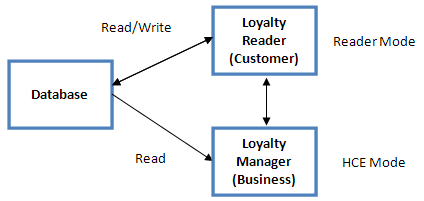
\includegraphics[width=0.48\textwidth]{img/dArch1.png}
   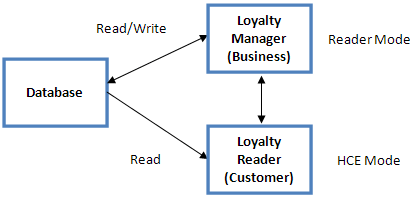
\includegraphics[width=0.48\textwidth]{img/dArch2.png}
    \caption{(i) Loyalty Manager using HCE. (ii) Loyalty Reader using HCE}
     \label{fig:dArches}
\end{figure}

\subsubsection{Loyalty Manager using HCE}
Loyalty Manager with HCE entails using the Manager application as a smartcard. In this case, the Loyalty Reader interfaces with the database to update the user's Stampbook. 

The benefits and drawbacks of this configuration are: 
\begin{description}[leftmargin=!,labelwidth=\widthof{\bfseries small}]
    \item[+] Syncing is not necessary as the Reader will always have the updated Stampbook
    \item[+] Less logic required in the Applications to direct stamps
    \item[---] Dependant on both applications having internet connection
    \item[---] The user must have the Loyalty Reader open to collect stamps
    \item[---] Data integrity issues if people maliciously modify code of the Reader
    \item[---] Differentiating between  reward \& stamp requests is difficult
\end{description}
\subsubsection{Loyalty Reader using HCE}
When the Loyalty Reader acts as the smartcard, several interactions differ. Primarily, the burden of dealing with the database is placed onto the Loyalty Manager.

The benefits and drawbacks of this configuration are: 
\begin{description}[leftmargin=!,labelwidth=\widthof{\bfseries small}]
    \item[+] The Loyalty Reader does not need to have the application open to collect a stamp, the phone functions as a passive smartcard.
    \item[+] Only the Loyalty Manager needs access to the internet. Customers will be able to collect and expend stamps whilst not connected
    \item[+] The Loyalty Manager can easily separate stamp requests from reward requests
    \item[+] Data is more secure as only the authorised Loyalty Manager has access to modify the database. Ultimately, this prevents user tampering and ensures data integrity within the system
    \item[---] Complex logic required in both applications
    \item[---] Providing specific feedback directly to the Loyalty Reader via the app is difficult
\end{description}

\subsubsection{Chosen Model}
Loyalty Reader using HCE was selected on the merit of its positives. Primarily, not requiring internet access from the customer, the ability to collect stamps without having the application open and its emphasis on security. On the other hand, it makes the implementation trickier, requiring more logic to support the two-way communications. None-the-less, we expect that this model will ultimately benefit the system by making it easier to use and understand for users.

\subsection{Design Methodology}
In order to develop the designs for the system components, we b
\subsubsection{Design Language}
One of Neilson's heuristics is `Consistency and Standards'~\cite{jakob}, in this case meaning that the solution should follow the platform conventions and design of the Android operating system. This was captured in the requirement S1. If this heuristic is met, users will feel more comfortable as the system presented to them feels familiar to use. The latest standards outlined by Google describe \emph{Material Design}~\cite{materialDesign}, a visual design language to be used with the new \emph{Android Lollipop} operating system with a goal to:
\begin{quote}
    \textit{``Develop a single underlying system that allows for a unified [user] experience across platforms and device sizes''}~\cite[Introduction]{materialDesign}
\end{quote}


\subsection{Design Process - Systems}

\subsubsection{Wire-Frame Mockups}
INSERT ORIGINAL DRAWN MOCKUPS HERE
\begin{figure}[H]
 \centering
  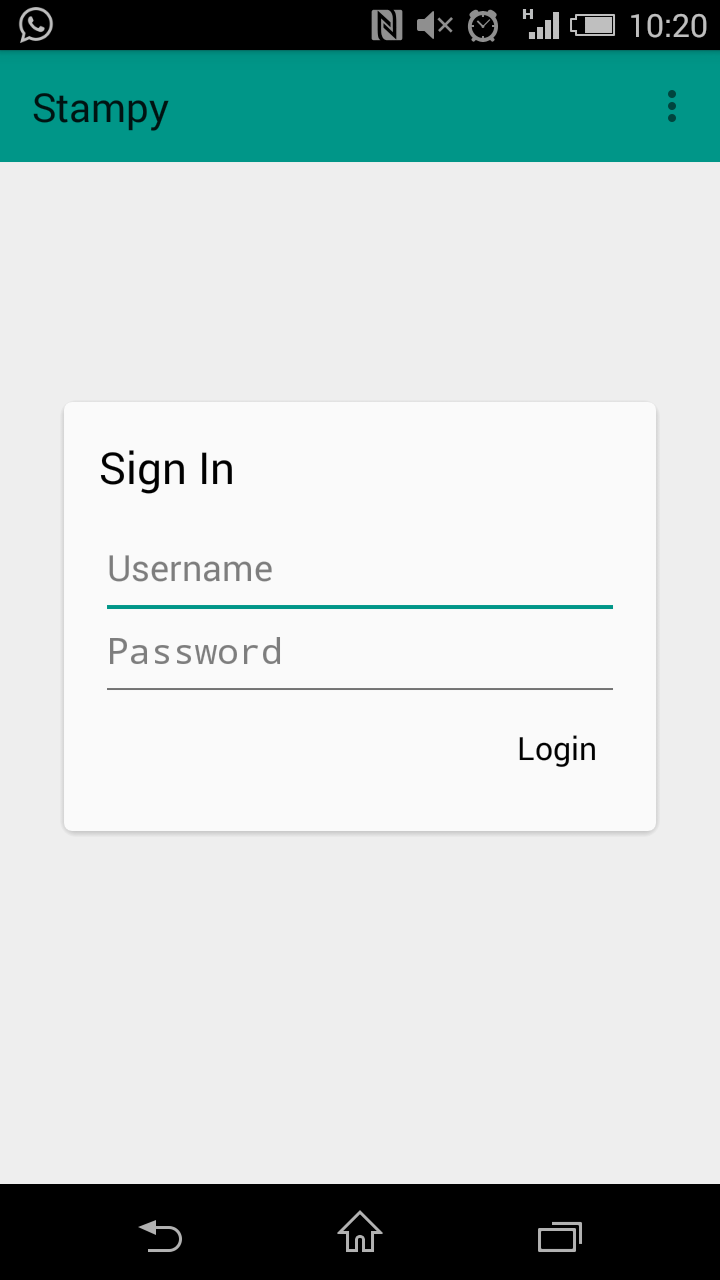
\includegraphics[width=0.24\textwidth]{img/loginMockup.png}
   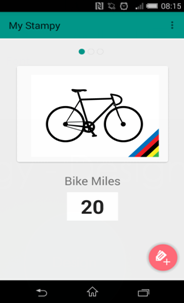
\includegraphics[width=0.24\textwidth]{img/MainMockup.png}
    \caption{Prototype}
\end{figure}

\textbf{Overview}
\subsection{Participatory Design}
\subsubsection{Need for Study/Problems With Guidelines}
\subsubsection{Aims}
\subsubsection{Outline}
\subsubsection{Results}

\subsection{Database Design}
\begin{figure}[H]
  \centering
    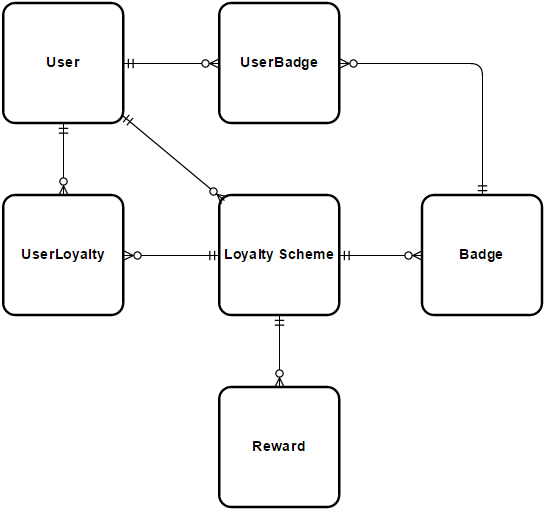
\includegraphics[width=0.5\textwidth]{img/erd.png}
      \caption{Entity Relationship Diagram}
\end{figure}
\begin{figure}[H]
  \centering
    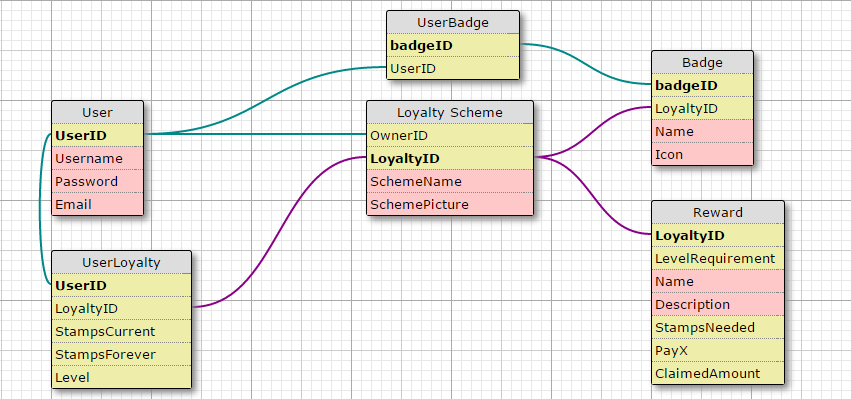
\includegraphics[width=1\textwidth]{img/architecture.png}
      \caption{Database Model}
\end{figure}


\chapter{Implementation}
\section{Introduction}
In this chapter, we will present the different software components that were combined together to build our system. Problems with engineering and platform complexity will be highlighted, along with the process for solving them. The Android operating system brings many challenges with regards to development; however the goal is to explain those which are interesting when developing solutions relating to NFC. A basic knowledge of the Android platform will prove useful to fully understand this chapter.
\section{Primary Technology}
As explained earlier (blah blah reference), Stamped is to be developed on a popular mobile platform that supports the NFC standard, in this case Android. At this moment in time, developing a functional prototype for this system cannot be possible on another platform due to hardware and API limitations regarding NFC and Host Card Emulation. Expanding the solution to external platforms in the future will be difficult as it requires a rewrite with platform-specific code.
\subsection{Software}
Google provides a plethora of development tools in order to develop applications, one such tool is the development environment \emph{Android Studio}. This kit provides an Integrated Development Environment (IDE) in order to design, configure and program the system. Android programs are coded using \texttt{JAVA} -- therefore requiring an object oriented methodology. 

Different Android devices run different versions of the operating system. Corresponding to each operating system version, there exists an accompanying Application Program Interface (API) that introduces new features to the ecosystem. We want our application to have the highest compatibility, but still contain the required features in order to satisfy the requirements. \emph{Android 4.4 KitKat} is selected as this is when Host Card Emulation was initially introduced into the platform; however, this means that approximately 45\%~\cite{Androidusagestats} of Android users have an appropriate version of operating system to run Stamped.

\subsection{Hardware}
Complementing the above choice of software, we require accommodating Android devices for development. Two devices were selected, a smartphone and a tablet. The tablet will be used to implement the Stamped Manager application as businesses will ideally mount Tablets onto a table next to employees to use. On the other hand, the phone will be used for the Stamped application as this is the common device customers will be using the system with. Both devices run the latest \emph{Android 5.0 Lollipop} operating system - therefore supporting Host Card Emulation. 

\section{Other Notable Resources}
\subsection{Webserver with Database}
To facilitate the backend of the system, we introduced a webserver/database backend in the design. A private webserver was purchased in order to facilitate the interactions with the database. The design database schema (Ref. SCHEMA) was imported into \emph{PHPMyAdmin} and PHP files were developed to interface between the Applications and Webserver (The rationale for this can be found in (Sec. \ref{sec:databasecommunication}))

\subsection{Android Debug Bridge (ADB)}
Google provides a useful software for application testing called The Android Debug Bridge. This software interfaces with connected devices, providing the following features.
\begin{itemize}
 \item The ability to see the console of the Android device in real-time whilst running the software
  \item The ability to control in-ward and out-bound network connections
   \item Error identification and debug output
\end{itemize} 

ADB persists whenever there is a connection between Android Studio and a device, outputting feedback on its current state.

\section{Implementation Complications}
In this section a discussion follows the key implementation complexities whilst developing the system. Care was taken to abstract the problems of developing on the Android platform away from the issues.
\subsection{Host Card Emulation}
We earlier defined a need for an interaction architecture, identifying the Stamped application to interact using HCE as a smartcard. In order to do achieve this, a service will need to be created 

\newpage{}

\subsubsection{Creating The Service}
In order to provide functionality outside of an application, a `service' must be implemented. A service is simply a component of an application which constantly runs in the background -- Host Card Emulation is one such example of a component. In this case, the HCE service passively runs in the phone working memory, waiting to be triggered by an NFC Reader before sending a message. The purpose of having HCE in this form allows users to tap a reader to collect stamps \textbf{regardless of whether the application is open on the device or not}.

Android services must be carefully developed, as reckless design will lead to unwanted battery drain on the device. Fortunately Google provides a template class called \emph{HostApduService} for HCE, ensuring that the service is optimised for power consumption. 

\subsubsection{Distinguishing Actions}
A standard smartcard cannot tell what exactly is being read from it or when, a similar problem presents itself in the Host Card Service. The HCE service cannot atomically discriminate what message it needs to send, it can only react to an \texttt{onRead} event. To remediate this, we had to temporarily break the object oriented principle of encapsulation by introducing a shared global variable \texttt{NFCMessageType}. The message will allow the Manager application to discriminate what type of action we are broadcasting as a smartcard. Two such messages are adopted:
\begin{enumerate}
 \item Stamp mode - Broadcasts the user account id
  \item Reward mode - Broadcasts the user account id, the scheme id and the number of stamps to deduct in order to claim that reward
\end{enumerate}
Passively the device is on `Stamp' mode; however once a user selects a reward, they are presented with a popup (Fig. \ref{fig:extrinsicmotivation}) to tap the reader in order to claim their reward. During this time, the HCE service will be in `Reward' mode. As the popup is dismissed (from tapping the reader or having the user press cancel), we return back to Stamp mode. This technique underlies the systems ability to Understand Actions (Sec. \ref{sec:understanding}).

\begin{figure}[H]
 \centering
  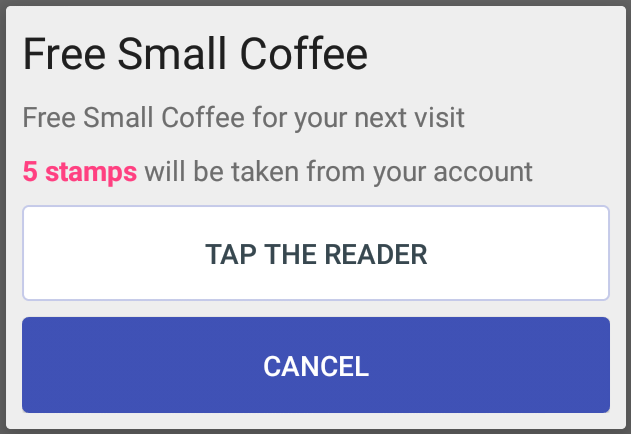
\includegraphics[width=0.40\textwidth]{img/claimreward.png}
     \caption{The popup presented to the user when they are about to claim a reward}
     \label{fig:claimreward}
\end{figure}

\subsubsection{Reacting to OnRead}
The \texttt{onRead} function is usually strictly used to send a message to a reader. However, the event affords many opportunities for us to implement user feedback mentioned in the design chapter. For instance, we announce to the user whenever they have tapped their device using audio feedback and a notification (Fig. \ref{fig:notification}). This novel solution binds the interaction feedback to the service; therefore these functions can run in the background.

\begin{figure}[H]
 \centering
  
\includegraphics[width=0.40\textwidth]{img/notification.jpg}
     \caption{A Notification providing feedback to the user upon receiving a stamp}
     \label{fig:notification}
\end{figure}

\subsection{NFC Communications}
Several presentation methods need to be put in place to facilitate NFC communication for our system. The messages being sent are simply hexadecimal plaintext; therefore there needs to be a way to send them in the correct format and carry some meaning to them. Here we demonstrate the principles to enable the Stamped Manager to understand messages.

\subsubsection{Understanding Actions}
\label{sec:understanding}
The Stamped Manager must be able to distinguish the types of messages it receives. There are two kinds that it may encounter: A stamp request and a reward claim. We earlier explained two modes on the host card that send differing amounts of information. Likewise, the Manager was setup in order to analyse message content. If only the accountID was received, we know that Stamped Manager needs to provide a stamp, however when is presented with more information, the system recognises that a customer is claiming a reward and deducts the amount of stamps from their account.

\subsubsection{Avoiding the `Beam'}
Android Beam is a feature of the Android platform to allow peer-peer data exchange over NFC~\cite{androidBeam}. Though it may have its uses (i.e Sending contacts, pictures), it can cause many problems for our system. Primarily, when two devices `tap', the operating system may mistake it for a `Beam' instead of a smartcard. This feature can be seen in (Fig. \ref{fig:androidBeam}); however we draw attention to the message which says `Touch to beam'. When this message appears, any input to the device other than that specific action is blocked. This will naturally clash with the Stamped Manager, which is expecting a host card message instead of a `Beam'

To solve this problem, we had to implement tight controls over how the Manager enables and disables its NFC chip, only enabling the chip whilst the reader is listening for a message from a host card.

\begin{figure}[H]
 \centering
  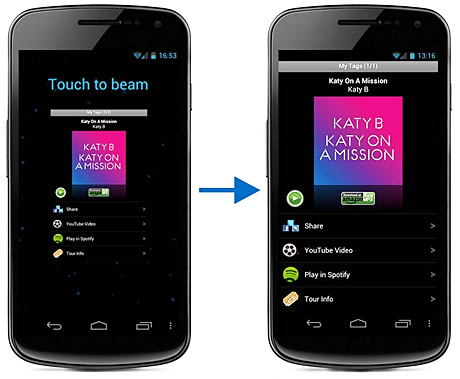
\includegraphics[width=0.40\textwidth]{img/androidBeam.jpg}
     \caption{A demonstration of Android beam}
     \label{fig:androidBeam}
\end{figure}

\subsubsection{ApplicationID Filtering}
An Android device can emulate many smartcards simultaneously; however this is an issue for a NFC Reader as it will not be able to distinguish between the smartcards. We solve this issue through ApplicationID (AID) Filtering. Whenever a host card is setup, an ApplicationID must be assigned to it in the form of a hexadecimal string. An NFC Reader application can apply an AID filter with a matching hexadecimal string (Fig. \ref{fig:aidfilter}) in order to identify and accept only the intended smartcard.

\begin{figure}[H]
 \centering
  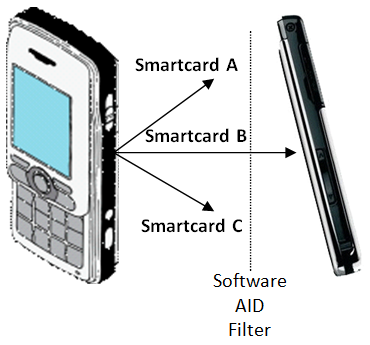
\includegraphics[width=0.40\textwidth]{img/aidfilter.png}
     \caption{A schematic demonstrating software AID Filtering}
     \label{fig:aidfilter}
\end{figure}

\subsection{Database Communication}
\label{sec:databasecommunication}
A large part of the system interactions involve reporting back to the central database in order to sync `stampbooks' along with user profiles. We deduced during the design stage that only the Stamped Manager will have access to modify entries in the database, whereas the user Stamped application will only be able to read from it -- A discussion follows on the implementation of database communication for our system.
\subsubsection{PHP Interface}
Interfacing directly with SQL is highly difficult and insecure in the Android platform. To solve this a new interface had to be made using PHP. In this architecture, applications send \texttt{GET} and \texttt{PUT} requests to the server, identifying actions by using `tags'. PHP in turn works as an intermediary, sending input to the database and providing output back to the Android application. Unfortunately this means that functions have to be written essentially twice, as they need to be written in JAVA to call a PHP, along with being written PHP to handle the input/output.
\subsubsection{Database Requests}
%UI THREAD NONONO
Requests to the database take time, and therefore must be threaded properly on mobile platforms. Android is very strict with regards requests what is allowed to run on the UI Thread. Requests that are recognised to be time consuming (i.e. Database requests) must be setup to run on a separate thread of execution. The adverse side effect of this requirement introduced the problem of race conditions in our UI.
\subsubsection{Dealing With Race Conditions in the UI}
Consider the following example -- A user is syncing their `stampbook' to see how many stamps they have for each of their loyalty schemes. The request runs in a background thread; however it does not update the new stamp values as they have already been drawn on screen. We fix this by constantly updating the views every few seconds. This solution was not ideal, nonetheless it did remediate our race conditions.

\newpage

\subsection{Internal Database Management}
Storing information on Android can be non-intuitive. Basic credentials can be cached through plain text files; but in order to store the complex inter-relating data of our system. An internal database needs to be deployed to serve as local storage. Here we outline the novel challenges when working with both an internal and online database.
\subsubsection{The Internal Database}
Information gathered from querying the online database has to be stored somewhere, as a result, a \texttt{SQLite} database is setup with an identical schema. The idea is to have a clone of the parts relevant to the user (i.e. Account details, loyalty schemes, available rewards) of the online database stored locally. This vastly reduces the number of database calls that need to be made, as well as solving our information storage problem. On the other hand, it adds an extra layer of complexity as some SQL queries will still need to be run on the internal database \textbf{as well as} the online database. 
%Syncing between Internal and Online backup
\section{Delivery of Requirements}
Here we will compare how well the implemented system delivered on our earlier requirements.

\subsection{Overview}
Here we show a high-level overview of how many MoSoCoW requirements were completed. 
\begin{itemize}
	\item Must Have -- 7/7
	\item Should Have -- 3/6
	\item Could Have -- 5/7
	\item Wont Have -- 0/2
\end{itemize}

\subsection{Requirement Fulfillment}
\begin{description}[leftmargin=!,labelwidth=\widthof{\bfseries Medium}]
    \item[M1] \textbf{Sign-In \& Registration} \newline
        \textit{Users are able to sign-in to the system with their accounts}
        
    \item[M2] \textbf{Fast Stamping} \newline
        \textit{Stamping in the adopted design is pervassive; therefore no buttons on the user interface is needed. Any tap on a listening reader will provide a stamp.}
    
    \item[M3] \textbf{NFC Transmission} \newline
        \textit{Host Card Emulation is used to send messages over NFC.}
        
    \item[M4] \textbf{Online Syncing} \newline
        \textit{The system actively syncs the status of user `stampbooks' with the online database.}
        
    \item[M5] \textbf{Sync on Interaction} \newline
        \textit{The \texttt{onRead} event triggers a sync with the database whenever an interaction between two devices take place}
        
    \item[M6] \textbf{Syncing Time} \newline
        \textit{A fast backend and grouped data in the \texttt{JSON} format affords fast syncing.}
        
    \item[M7] \textbf{Feedback on Interaction}
        \textit{The system provides an audible sound and a notification whenever an interaction occurs.}

    \item[S1] \textbf{Consistency} \newline
        \textit{The system user interface was implemented using Google's Material Design.}
        
    \item[S2] \textbf{Rewards Browsing} \newline
        \textit{There is a dedicated rewards tab to allow users to browse all available rewards for a loyalty scheme.}

    \item[S3] \textbf{Badges} \newline
        \textit{Users are able to collect standard badges which earn a user `title'.}
     	
    \item[C1] \textbf{Passive Card Emulation} \newline
        \textit{The system does use passive host card emulation.}

    \item[C2] \textbf{Branding} \newline
        \textit{Some customisation options are available to schemes; however no frontend for them was implemented}

    \item[C3] \textbf{Internet-Free Stamping} \newline
        \textit{Only Stamped Manager requires an internet connection in order to provide a stamp. Customers can sync their stampbook whenever they have an internet connection to update their local stampbook.}
        
    \item[C4] \textbf{Multiple Device Support} \newline
        \textit{Having an online database affords the use of using your account on multiple devices - moreover they will be synced with eachother}
        
    \item[C5] \textbf{User Personalisation} \newline
        \textit{Our system allows the personalisation of profile pictures and user-earned `titles'.}
\end{description}

\newpage

\section{Design Conformance}
By following the criteria laid out in the design chapter, we managed to successfully produce two android applications which allow users to do the following:

\begin{enumerate}
	\item Collect stamps for corporate loyalty schemes
	\item Track progress of all loyalty schemes in real-time
	\item Expend stamps in order to claim rewards
	\item Collect badges to improve customer engagement
\end{enumerate} 

\section{Conclusion}
Throughout this chapter, we have concentrated on implementing a system in order to meet our requirements and design specifications. In the next chapter, we will introduce and perform a user field study to assess the system in a naturalistic environment.

\chapter{Evaluation}
\section{Introduction}
This chapter outlines the process for evaluating the system, describing a field study in a naturalistic environment 
\section{Field Study - Observation of The System In a Natural Environment}
\subsection{Outline \& Objectives}
The primary purpose of our study is to identify the contribution of gamification on the system: whether it improves or hinders user engagement \& enjoyment. To quantify the value of gamification in the system, we use an A/B Testing~\cite{ABTesting} approach. This involves comparing two near-identical versions of the system with the exception of a single variation, allowing us to measure the impact of said variation on user behaviour. As such two systems were implemented \textbf{`System A' (without gamification)} and \textbf{`System B' (with gamification)}. 

\subsection{Study Methodology}
There exist two applicable methods to evaluate our system, laboratory and field studies. We can define a laboratory study as:
\begin{quotation}
\noindent
`A research study conducted in a contrived setting in which the effect of all, or nearly all, influential but irrelevant independent variables is kept to a minimum.''~\cite[p.~215]{marketStudy}
 \end{quotation}

Lab experiments are preferable in situations where the environment and variables need to be controlled. The outcome of this method is data specific to what you want to test. On the other hand, the controlled surroundings may ignore not reflect the use of the system in a wider general context.

Oppositely, a field study is:
\begin{quotation}
\noindent
``A research study conducted in a natural setting in which one or more independent variables are manipulated by the experimenter under conditions controlled as carefully as the situation will permit.''\cite[p. 211]{marketStudy}
 \end{quotation}

The advantage of a field study is the ability to test the system in a natural environment, allowing us to deal with the exact same environment where the system would be used. On the other hand, we have less control of the external variables, which may introduce `confounding variables'\footnote{Confounding variables directly or indirectly link the dependant and independent variables.} that can negative affect the studies external validity~\cite{fieldstudysux}.

\subsubsection{Selected method}
A field study was selected as we want to see how a novel way of collecting loyalty stamps works in the real world. We can see how users learn to use the system throughout the study. Not having control of the environment can prove advantageous as we can isolate and attempt to remediate any negative variables that are caused by `natural use'. A pilot study (to be discussed in Sec. xx) will need to be performed in order to identify some of these initial variables.

\subsection{Demographics}
Six participants were recruited that owned a compatible Android device (Android 4.4 KitKat+) for our system. An even amount of male and females were recruited eventhough women tend to frequent loyalty schemes more often than men~\cite{womenloyalty}. All participants were students within our target demographic of 16-40, having the average age of 21.5.

\subsection{Preparation}
Two systems were prepared for the study --- `System A' (without gamification) and `System B' (with gamification). The primary functionality of both systems are identical except for the addition of badges/quests to System B. Participants were evenly assigned a system to test at random. We required users to install the application on their own device to ensure the system works with a variety of hardware. 

An example loyalty scheme `Bath Cafe' was setup for the study (Fig. \ref{fig:bathcafe}). It was designed in such a way that users will be able to claim at a free coffee by the end of the study.

\begin{figure}[H]
 \centering
  
\includegraphics[width=0.40\textwidth]{img/bathcafe.png}
     \caption{The example loyalty scheme to be used in the study. A reward of a free coffee is offered upon completing the stamp card.}
     \label{fig:bathcafe}
\end{figure}

An accompanying badge was created for the loyalty scheme, as can be seen in Fig. \ref{fig:badge2}. The badge was purposefully simple to collect in order to be attainable throughout the study.

\begin{figure}[H]
 \centering
  
\includegraphics[width=0.50\textwidth]{img/badge2.png}
     \caption{A badge implemented for the study. Both the badge and the `connoisseur' title unlock when a user claims their first coffee.}
     \label{fig:badge2}
\end{figure}
 
Three coffee shop locations were identified on a university campus to perform the field study. A random location was to be visited on each of the five days. At each location a business employee will be asked to use the `Stamped Manager' application to facilitate our study.
 
\subsection{Developing The Questionnaire}
The primary method of gathering quantitative data from this study is using a questionnaire, complimented by some comment questions to gather further qualitative data for their answers.

We prepared two questionnaires, one for the participants to complete upon finishing the study and one for a coffee shop employee to fill-out at every unique location visited for the study. An explanation of their purpose follows:

\subsubsection{Questionnaire For Users}
The user questionnaire attempts to quantify the participant's loyalty scheme patterns and their response to the application and technology. To achieve this, the questionnaire was broken down into several sections.
\begin{itemize}
	\item \emph{Questions 2 \& 3} informs a participants behaviour regarding loyalty schemes. Having a wide variety of loyalty scheme behaviours allow us to get a complete range of opinions regarding our system.
	\item \emph{Question 4} was introduced from the Technology Acceptance Model (TAM)~\cite{tam} (Fig. \ref{fig:TAM}). The TAM models how individuals accept and use new technology based on `perceived usefulness' and `perceived ease of use' factors--- satisfying these variables predicts a system that is more likely to see use~\cite{tam}.
	\item \emph{Question 5} one way in which we can gauge how much participants enjoyed using the system is to identify whether the participant would recommend the system to friends. Furthermore, personal use also indicates system enjoyment.  
	\item \emph{Questions 6 \& 7} Are specific to the tested system, only one of them requiring an answer. By asking these questions, we aim to understand what potential impact, positive or negative, gamification can have on the system. 
	\item \emph{Question 8} Requires users to provide qualitative feedback about their experience. We ask for positives and negatives in order to encourage a balance in the answers, along with suggestions for system improvements.
\end{itemize}

Whereas question 4 is designed to measure user trust in the system (whether users will use the system), questions 5, 6 and 7 are to be used to measure our hypothesis.

\begin{figure}[H]
 \centering
  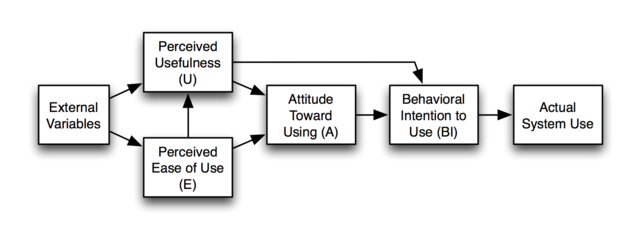
\includegraphics[width=0.80\textwidth]{img/TAM.png}
     \caption{The Technology Acceptance Model (TAM) modelling the link `perceived usefulness' and `perceived ease of use' has on system use }
     \label{fig:TAM}
\end{figure}

\subsubsection{Questionnaire For Business}
The business questionnaire is designed to give context to the location where a field study is being performed. The questions mainly identify what type of loyalty schemes exist within that business, the rewards they give and the percentage of customers that participate in them. Finally there is an option for employees to provide feedback on the Stamped Manager. Effort was made to keep this questionnaire as simplistic as possible to ensure minimum disturbance of the employees.

\subsection{Pilot Study}
A pilot study allows the identification of correct processes and captures any small issues that may affect the primary field study. The primary purpose of the pilot is to assess the interaction using the application on a participant's phone.

A separate participant was recruited. She described limited-to-no knowledge of mobile technologies and was a casual consumer of smartphones. They were told to download and install Stamped, whilst we installed the Stamped Manager on a tablet device. A list of tasks was generated in order to test the `interaction elements' (stamping/reward claiming) of the applications. In the interest of time, we designed the tasks to be completed in one sitting.

The list of tasks were as follows:

\begin{enumerate}
  \item Login to the system using your university email and password `1234`
  \item Ensure your phone is unlocked (you do not need to have the application open) to collect a stamp
  \item Tap your phone onto the reader when asked (you will be given 5 stamps)
  \item Click on the notification/open the application
  \item Ensure you received 5 stamps in the loyalty scheme `Bath Cafe`
  \item Swipe to the profile page
  \item Confirm that you have 1 available reward on your profile page
  \item Swipe to the rewards tab
  \item Select the available reward `free coffee`
  \item Notify the researcher that you want to claim a reward
  \item Tap your phone onto the reader when asked
  \item Open swipe to your schemes and ensure the stamps have been deducted
\end{enumerate}

\paragraph{Findings}

The user was proficient at navigating the application, a tabbed interface proved to be easy for them to understand. Several user interface bugs were also quickly discovered, such as no feedback when a user tries to login with incorrect credentials. These were corrected before the main study took place.

Some questions on the questionnaire were deemed to be confusing and had to be revised for the future study. 

Various hardware-level issues were identified that intruded with the interaction. Different phones have their NFC Chip located in various places, making it difficult to know where users should tap their device. There were points where they were sliding the back of their phone on the tablet in attempt to trigger the interaction. Moreover, we identified that using a very thick protective `phone-case' (as the participant had), limited some NFC signal.

Positioning the tablet on the stand was a problem. The stand put the device at an awkward angle on table with regards to the user, making it difficult to tap the back of the device with a smartphone. Furthermore the awkward angle sometimes caused a `weak NFC interaction'\footnote{A weak NFC interaction occurs when an NFC interaction is interrupted mid-way, thus one device fails to communicate its message, whilst the other believes it has taken place.}, providing unintended feedback that would trick users into thinking that an interaction has occurred.

\paragraph{Solutions}

As a majority of the issues were hardware orientated, several process solutions were implemented to remediate them for the main study. Firstly for future participants, we checked if their phone-case was not too thick, asking them to remove it for the purpose of the study if necessary. Secondly they were instructed to `swipe' along the back of the tablet instead of a simple tap to ensure the NFC interaction completes. 

The ideal solution for this problem would be to purchase a USB-to-MicroUSB adapter and a standalone USB NFC reader for the Stamped Manager (Fig. \ref{fig:usbnfc}), having the user tap their smartphone on the reader instead. Using this configuration will not only correct the awkward angle/weak interaction problem, but will also provide NFC functionality to devices that do not have it available.  The flexibility of this solution would make it preferrable for businesses.

\begin{figure}[H]
 \centering
  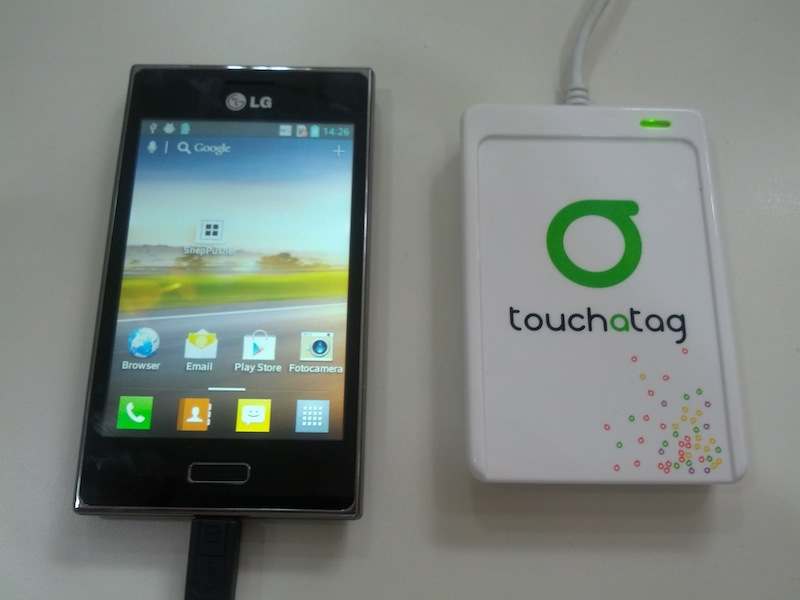
\includegraphics[width=0.4\textwidth]{img/nfcusb.jpg}
     \caption{A smartphone device connected to a USB NFC reader}
     \label{fig:usbnfc}
\end{figure}

\subsection{Hypothesis}
We clarify our hypothesis to be expanded on as \textbf{Hypothesis A: Participants using Gamification are more likely to enjoy to system and recommend it to friends}. We understand that `enjoy' is a very general term, and therefore attempt to quantify this by using questions 5, 6, 7 in our questionnaire as our dependant variables (Fig. \ref{fig:questionz}). Those with gamification should respond more positively to Q5 than those without. Moreover, participants should respond positively to the question unique to their system (Q6 or Q7).
\begin{figure}[H]
 \centering
  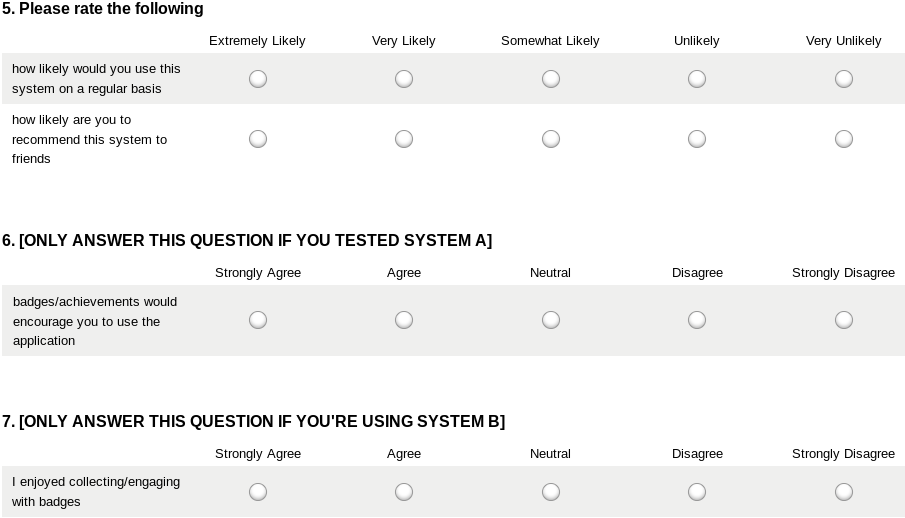
\includegraphics[width=0.81\textwidth]{img/questions.png}
     \caption{Questions 5, 6, 7 of our questionnaire to be used as our dependant variables}
     \label{fig:questionz}
\end{figure}
\newpage
\subsection{Approach}
Here we describe the process by which the study was performed. The researcher began by briefing the participants as per Fig. XXX on the context and purpose of the project. They were guaranteed that the system is being tested rather than themselves, along with the confidentiality in their responses by storing no personally identifying information. Participants were then required to download and install their assigned system onto their smartphones (Fig. \ref{fig:fieldstudyfamily}) --- instructions can be found in appendix XXX. Finally, they were asked to sign a permission slip, an example of which can be seen in Sec. XXX.

The main directive given to the participants is that they must collect stamps throughout the study, claiming a free coffee once they have accumulated enough of them. Those testing System B (with gamification) were directed to ensure that they collect the badge by the end of the study. 

\begin{figure}[H]
 \centering
  \includegraphics[width=0.60\textwidth]{img/fieldstudyfamily.png}
     \caption{A photograph showing the three devices which used System B}
     \label{fig:fieldstudyfamily}
\end{figure}

We began the study by setting a convenient time to meet everyday in an earlier communicated coffee shop for the session. It was important to select a non-peak time as to minimise disturbance to the staff. All six participants were sat down and asked to wait; meanwhile the researcher asks the coffee shop employee to use the tablet with the Stamped Manager  for the next six people that ask for a `digital stamp'. They were assured that the stamps were only for a study and not legible --- this was followed by a quick training on how to use the Stamped Manager. The tablet was left on the till, ready for the employee to use to distribute stamps.
\newpage
Once training was completed, the participants were instructed to travel individually to perform a regular coffee shop transaction, claiming a digital stamp (or free coffee) from the employee. The interaction was two-way; employees have to press the appropriate button on the Manager (Stamp/Receive Reward), whilst the participants swipe their phone onto the back of the tablet (Fig. \ref{fig:hollystamping}). Meanwhile, the researcher sat down to observe the interactions between them. At the end of each session, the researcher would ask the employee to fill in the business questionnaire. Once all formal parts of the session were complete, participants were offered a cupcake for their troubles.

\begin{figure}[H]
 \centering
  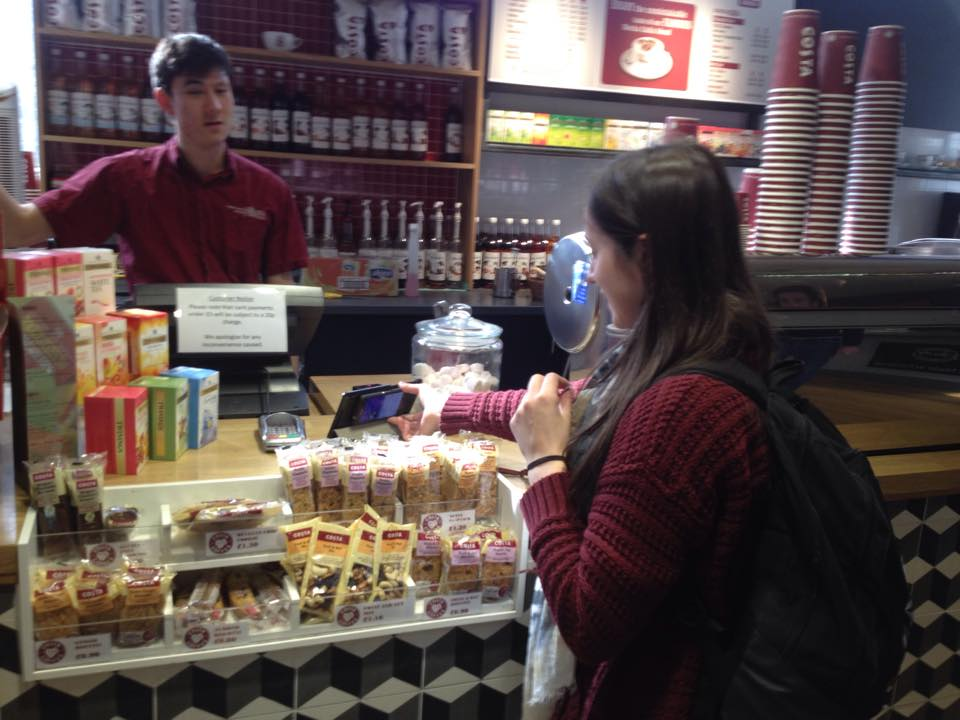
\includegraphics[width=0.6\textwidth]{img/hollystamping.jpg}	
     \caption{An photograph of the field study - a participant is seen claiming a stamp at the counter of a coffee shop}
     \label{fig:hollystamping}
\end{figure}

This format was repeated every day for five consecutive days (Monday-Friday), with each session lasting 10-20 minutes. By the end of the study, participants should have tested all three main interactions (stamping, reward claiming and badge receiving). Finally, upon confirming that all participants have completed their tasks, the post-study questionnaire was disseminated for them to complete.
 
\section{Conclusion}
This chapter outlined how our field study was conducted, along with the elements which we are trying to quantify. In the next chapter, we will discuss the findings of the study.

\chapter{Results \& Discussion}
\section{Introduction}
This chapter presents the results from our study outlined in the previous chapter, determining if the hypothesis introduced in the previous chapter (Sec. \ref{hypothesis}) is supporting. We determine the effects of gamification on our system, analysing qualitative user feedback to enrich the findings.
\section{Results of Study Outline}
We analyse the participants reactions to our system. For some aspects of the study where comparisons are needed, we split the feedback on a system basis. Unless otherwise specified, results are represented on an emotional scale from 1 -- 5 where 5 represents the most positive response and 1 represents the most negative.

The results can be seen in Table \ref{employeeGraph} and Figure \ref{participantGraph}. The participant graph only shows the metrics which were compared between systems. It is important to highlight that qualitative data is not reflected in these graphs; however the justification of individual replies lie in the qualitative responses --- these will be further discussed in Section \ref{sec:qualitative}.

\begin{table}[h]
  \resizebox{\textwidth}{!}{%
\begin{tabular}{@{}ll@{}}
\toprule
\textbf{Question}                                                 & \textbf{Responses}                                \\ \midrule
Does your business have a loyalty scheme?                         & Yes (3/3)                                         \\
What type of loyalty scheme do you run?                           & Stamp Card (2/3) | Reward Card{[}Barcode{]} (1/3) \\
What rewards can the customer claim using the loyalty scheme?     & Free Item (2/3) | Upgrade (2/3)                   \\
What percentage of customers do you feel take part in the scheme? & 40\%-59\% (1/3)|  60\%-79\% (2/3)                 \\ \bottomrule
\end{tabular}
}
     \caption{A table depicting the different type of loyalty schemes available at the locations the study was run in}
     \label{employeeGraph}
\end{table}


All visited coffee shops at the university campus had at least a paper-based stampcard set in place for a loyalty scheme.  A substantially large percentage of customers seemed to partake in the loyalty scheme (average of 75+\%). One location had a smartcard as well as a paper stampcard.

%Union loyalty scheme
%Most paperbased etc

\subsection{Participant Questionnaire}
\begin{figure}[H]
 \centering
  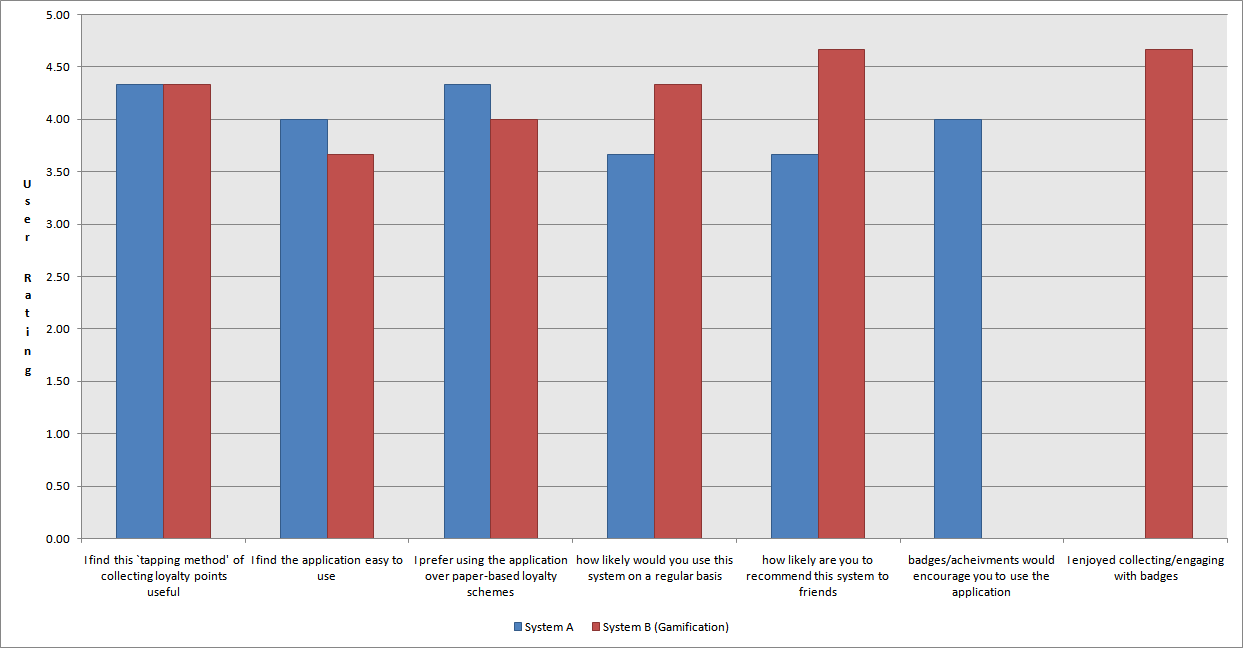
\includegraphics[width=1\textwidth]{img/graph.png}
     \caption{Results of the quantitive questions from the study that compared both systems}
	 \label{participantGraph}
\end{figure}

It is evident that questions regarding gamification have a strong positive average response (4+); however there are areas where System A marginally outperforms System B. These areas would be interesting for us to explore further. Both systems appeared to generally receive favourable responses from our participants.
\newpage
\section{Analysis of Questions}
In this section we analyse and discuss each question individually with regards to our hypothesis.
\subsection{Questions 1, 2, 3 --- Participant Loyalty Habits}
With these questions we aim to create a portrait of our participant's loyalty habits. We do not use this question to compare our hypothesis as these questions are systems independent--- the aggregated results for these questions are shown below in Table \ref{table:q123}
    \begin{table}[H]
    \resizebox{\textwidth}{!}{%
    \begin{tabular}{@{}llcc@{}}
    \toprule
    \textbf{Question}                                                           & \textbf{Average Response (s.d)} \\ \midrule
    Q1 – Age                                                                    & 21.67 (.577)                              \\
    Q2 - Gender                                                                 & 50\%/50\% Male/Female              \\
    Q3.1 - Stamps Collected Weekly                                              & 3.1 (.633)                             \\
    Q3.2 - I am more likely to complete a stampcard once I start collecting one & 4.0/5.0 (.633)                          \\
    Q3.3 - I occasionally forget/misplace my loyalty cards                      & 3.0/5.0 (1.265)                           \\ \bottomrule
    \end{tabular}
    }
    \caption{Table showing answers to questions 1, 2 and 3 from the study}
    \label{table:q123}
    \end{table}

As can be seen from the results, the average user collected 3.1 stamps per week.

There was a wide range of answers regarding forgetting/misplacing loyalty cards but generally 50\% of participants tended to forget/misplace their loyalty cards.

\subsection{Question 4 --- Technology Acceptance/Ease of Use}
This question measures user acceptance of our technology.  Responses are split between systems and can be found in Table \ref{table:q4}
    \begin{table}[H]
    \resizebox{\textwidth}{!}{%
    \begin{tabular}{@{}llcc@{}}
    \toprule
    \textbf{Question}                                                       & \textbf{Average Response (s.d)}                                                                       \\ \midrule
    Q4.1 - I find this `tapping method' of collecting loyalty points useful & \begin{tabular}[c]{@{}l@{}}System A - 4.33/5.0 (.577) \\ System B - 4.33/5 (.577)\\ Total - 4.3/5.0 (.408)\end{tabular} \\ \midrule
    Q4.2 - I find the application easy to use                               & \begin{tabular}[c]{@{}l@{}}\textbf{System A - 4.0/5.0 (.000)}\\ System B - 3.6/5 (.577)\\ Total - 3.8/5.0 (.516)\end{tabular} \\ \bottomrule
    Q4.3 - I prefer using the application over paper-based loyalty schemes & \begin{tabular}[c]{@{}l@{}}\textbf{System A - 4.66/5.0 (.577)}\\ System B - 4.0/5.0 (1.000)\\ Total - 4.33/5.0 (.816)\end{tabular}  \\ \midrule
    \end{tabular}
    }
    \caption{Table showing answers to question 4 from the study}
    \label{table:q4}
    \end{table}

    Participants agreed on the usefulness of the tapping method to collect stamp.

    Participants with System B found the system harder to use than those using System A.

	There are several explanations why addition of gamification seemed to make the application more difficult to use. Badges may have been implemented in such a way that clutters the interface, making it harder to use. On the other hand, by referencing the Technology Acceptance Model (Fig. \ref{fig:TAMagain}), the `easy to use' metric does not impact acceptance factors as much as perceived usefulness, they only affect the attitude towards using the system.  It is the `perceived usefulness' of the application that can directly affect the attitude and behavioural intention to use the system.
    \begin{figure}[H]
 \centering
  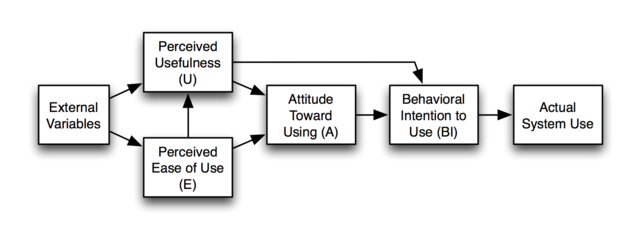
\includegraphics[width=0.80\textwidth]{img/TAM.png}
     \caption{The Technology Acceptance Model (TAM) displaying that `Perceived easy to use' has more impact on behaviour to use than `easy to use'}
     \label{fig:TAMagain}
\end{figure}

\subsection{Question 5 --- User Enjoyment/Recommendation}
This metric is one which we use to gauge user enjoyment of the system. Individuals who enjoy the system are more likely to use it themselves and recommend it to others. The feedback can be found in Table \ref{table:q5}.
    \begin{table}[H]
    \resizebox{\textwidth}{!}{%
    \begin{tabular}{@{}llcc@{}}
    \toprule
    \textbf{Question}                                                      & \textbf{Average Response (s.d)}                                                                            \\ \midrule
    Q5.1 - How likely would you use this system on a regular basis         & \begin{tabular}[c]{@{}l@{}}System A - 3.66/5.0 (1.154)\\ \textbf{System B - 4.33/5.0 (1.154)}\\ Total - 4.0/5.0 (1.094)\end{tabular}  \\ \midrule
    Q5.2 - How likely are you to recommend this system to friends          & \begin{tabular}[c]{@{}l@{}}System A - 3.66/5.0 (1.154)\\ \textbf{System B - 4.66/5.0 (.577)}\\ Total - 4.17/5.0 (.983)\end{tabular} \\ \bottomrule
    \end{tabular}
    }
    \caption{Table showing answers to question 5 from the study}
    \label{table:q5}
    \end{table}
    \newpage
   	Participants using System B were more likely to use the system on a regular basis and recommend Stamped to friends than those testing System A. Therefore,

	\textbf{Q5.1 Hypothesis supported}

	\textbf{Q5.2 Hypothesis supported }

\subsection{Question 6 \& 7 --- Gamification In The System}
Question 6 was exclusive to those that tested System A (without gamification), whereas question 7 was exclusive to System B (with gamification). The purpose of these questions is to get explicit feedback regarding our gamification elements--- results are shown below in Table \ref{table:q67}.
    \begin{table}[H]
    \resizebox{\textwidth}{!}{%
    \begin{tabular}{@{}llcc@{}}
    \toprule
    \textbf{Question}                                                  & \textbf{Average Response (s.d)} \\ \midrule
    Q6 - Badges/achievements would encourage you to use the application        & System A - 4.17/5.0 (1.000)                  \\ \midrule
    Q7 - I enjoyed collecting/engaging with badges					  & System B - 4.66/5.0 (0.588)                  \\ \bottomrule
    \end{tabular}
    }
    \caption{Table showing answers to questions 6 and 7 from the study}
    \label{table:q67}
    \end{table}

    Question 6 asked participants using System A how much value they would perceive badges/achievements would add to the system.

    Question 7 explicitly asked participants if they enjoyed the gamification elements included in the application and whether they gained value in engaging with them.

    In both systems, responses were far more positive in System B than System A, therefore,

    \textbf{Q6 - Hypothesis supported}

    \textbf{Q7 - Hypothesis supported}

\section{Analysis of Qualitative Feedback}
\label{sec:qualitative}
Here we analyse qualitative feedback that was gathered from both the questionnaire and general responses
\subsection{Researcher Observations}
Accompanying the participant responses, the researcher aggregated findings from observing the participants over the study --- these are discussed in terms of how predicatable the interaction was and if the application needed to be open when stamping.
\subsubsection{Predictability of the Interaction}
As earlier identified in chapter 6, `weak NFC interactions' is an issue caused by several factors. We attempted to mitigate their occurance by changing the way we instruct participants to tap the reader. Nonetheless, at every meeting at least one weak interaction occurred with participants. Though this is a high-priority issue that needs resolving in the future, we predict that implementing the solution below would greatly reduce the rates of weak interactions.

\paragraph{Ideal Solution}

The ideal solution for this problem would be to purchase a USB-to-MicroUSB adapter and a standalone USB NFC reader for the Stamped Manager (Fig. \ref{fig:usbnfc}), having the user tap their smartphone on the reader instead. Using this configuration will not only correct the awkward angle/weak interaction problem, but will also provide NFC functionality to devices that do not have it available.  The flexibility of this solution would make it preferrable for businesses.

\begin{figure}[H]
 \centering
  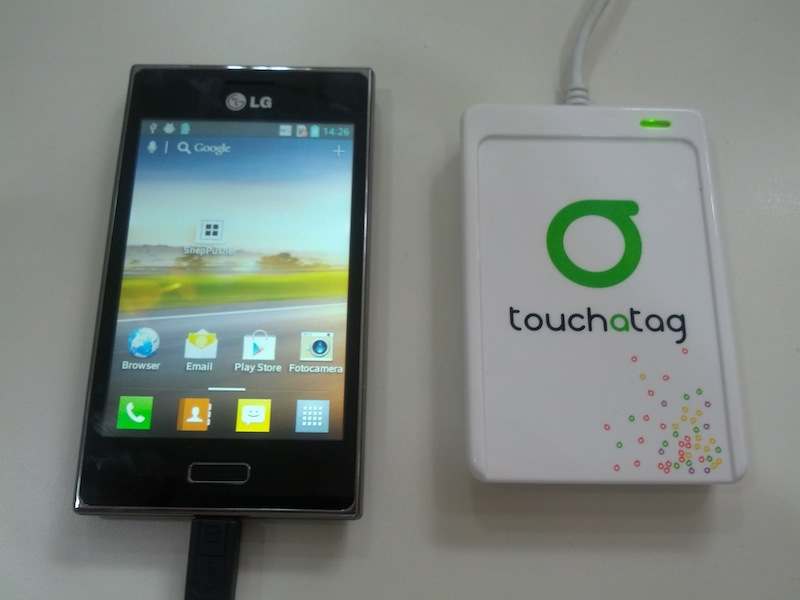
\includegraphics[width=0.4\textwidth]{img/nfcusb.jpg}
     \caption{A smartphone device connected to a USB NFC reader}
     \label{fig:usbnfc}
\end{figure}

\subsubsection{Keeping the Application Open To Stamp}
Although Host Card Emulation does allow users to collect stamps without having the application open, almost all participants chose to have the application open when tapping the reader. When questioned on the matter, one participant suggested that they trusted that the interaction would complete more reliably if they had Stamped open. This is primarily due to Host Card Emulation running in the background on the device, therefore making it difficult for users to tell if the service is running whilst the application is not open.

One participant mentioned that he wanted to tap the reader without having the screen on/application open. Unfortunately implementing this suggestion as a solution would have a massive negative impact on battery life and therefore, is not a preferable.
\subsection{Gamification Feedback}
The general response towards gamification was strongly positive. Several individuals suggested adding more meaning to the badges as they seemed to mainly serve aesthetic purposes; nonetheless   a potential solution is discussed in Sec. \ref{sec:invite}.

Asking participants that tested System A their opinion about adding badges proved to be very interesting. As System A participants never get to see the system with gamification, their perception would be of `their ideal implementation' instead of our own. More specifically, if they cannot imagine the value gamification adds to their system in their imaginary implementation, then it may not be useful to have at all.

One individual who tested System A highlighted that the gamification would be redundant as a motivator. When questioned why, they said that there already exists motivations to use the system in order to reap the rewards of loyalty schemes; therefore the addition of gamification would seem to be `bolted on'. This is a valid criticism of our implementation as there is no direct link between gamification and the loyalty schemes themselves. We can remediate this in several ways, firstly by allowing the creation of more complex badges (e.g. Visit all loyalty schemes in an area) and secondly, deeply integrating gamification principles to the rewards themselves; for instance allowing users to level up their loyalty schemes for better rewards.

\section{Limitations of Study}
This section outlines several factors which limited our study.

The number of participants could have been increased; however a key requirement of participants for our study was an Android phone of a compatible version to run Stamped. Moreover running field study sessions with all participants present would become a logistically strenuous task. One solution to counteract this would be to test the system in a different context (i.e. Gym passes, Bike Miles etc).

Only a single type of gamification was tested for our A/B testing, meaning that our results may not suggest positive response to gamification as a whole but only to our specific implementation of badges.  A different way to run the study would be to have three control groups, System A with no gamification, System B with Badges and System C with a different type of gamification. This would allow us to get a more holistic feedback on gamification in our system, as well as the gamification technique users prefer.

In terms of analysing user reactions to gamification, it can be difficult to ask users how they feel about adding badges into the system if they tested the system without them. On the other hand, this questions users regarding whether they would see value in its implementation. %idealistic

\section{Feedback on the Final Designs}
Throughout the process of design to the evaluation, feedback was gathered on the final design of the Stamped (Fig. \ref{fig:wireframer3}) and Stamped Manager (Fig. \ref{fig:wireframemr2}). In the interests of time, we will not perform any further iterations on the system design; however this feedback will be vital for future work.
\subsection{Stamped}
\begin{figure}[H]
 \centering
  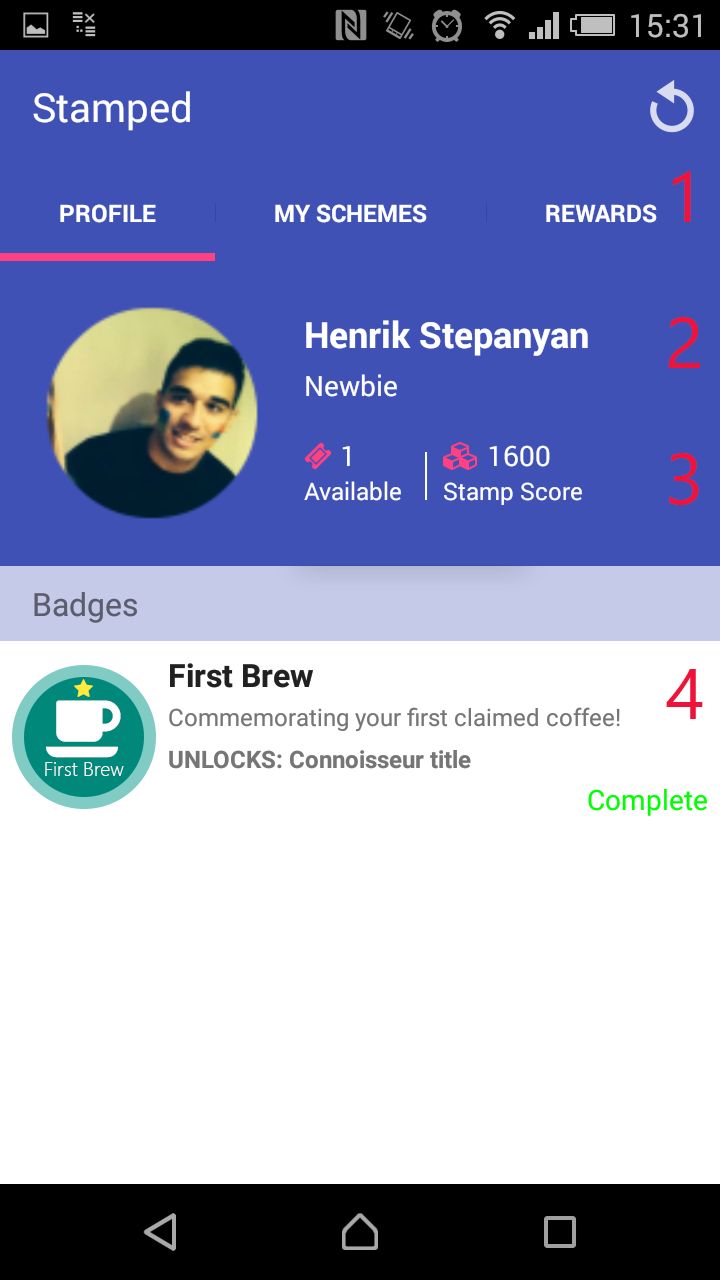
\includegraphics[width=0.275\textwidth]{img/moremock2.png}
   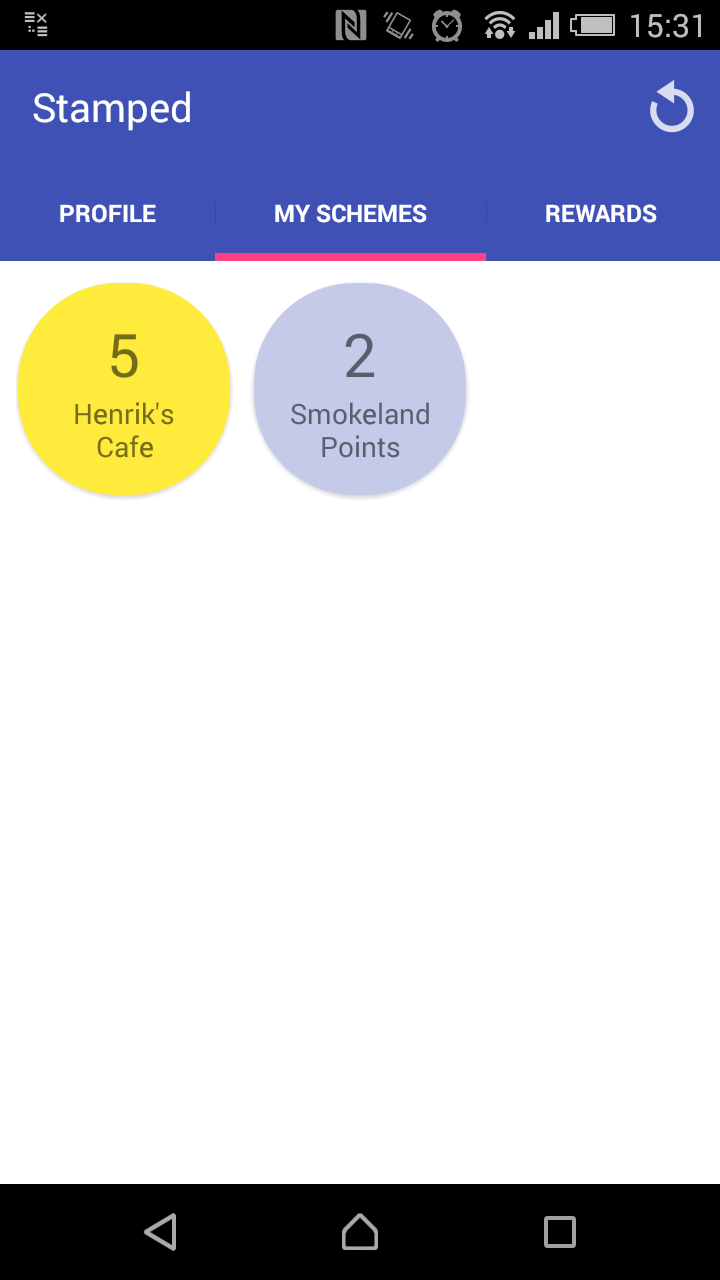
\includegraphics[width=0.275\textwidth]{img/finalmock.png}
    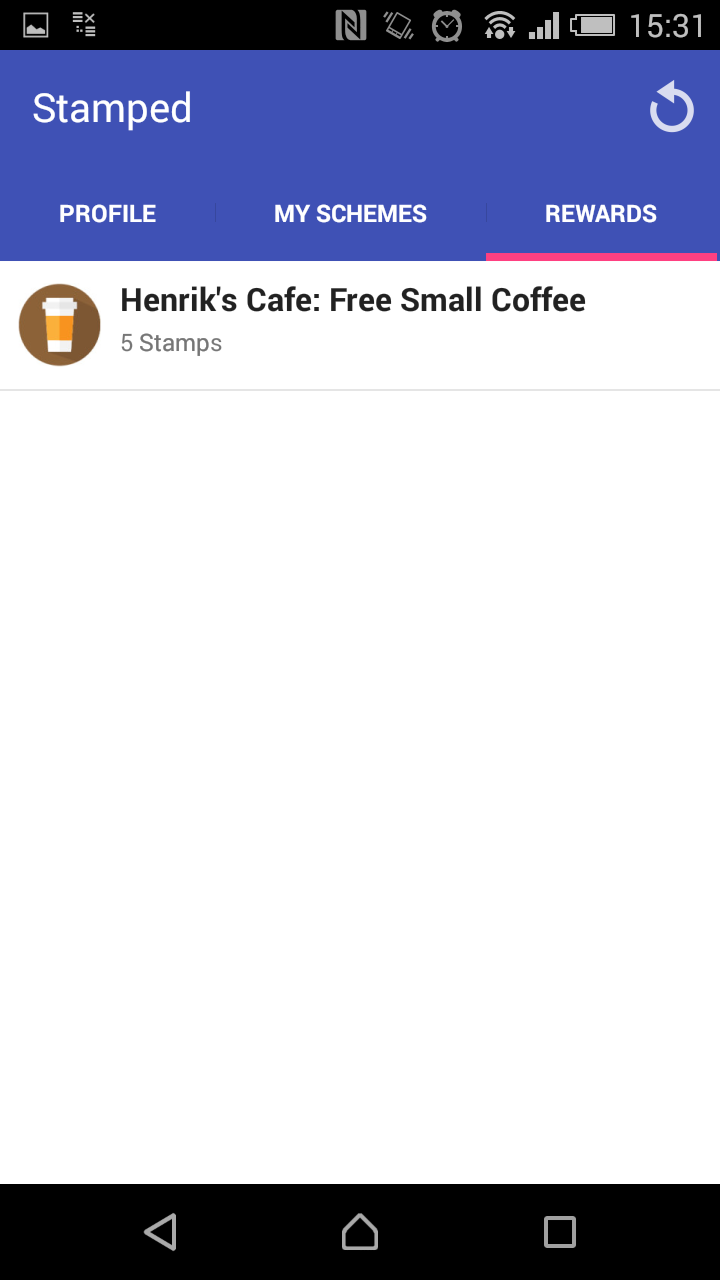
\includegraphics[width=0.275\textwidth]{img/moremock1.png}
     \caption{The final design of Stamped with a tabbed interface}
     \label{fig:wireframer3}
\end{figure}

\subsubsection{Feedback For Next Iteration}
The design was present to three potential users individually, along with all participants during the evaluation. A list of their suggestions follows:
\begin{itemize}
  \item \textit{``There should be more room for businesses to customise their schemes according to their brand''}
  \item \textit{``Single rewards per loyalty scheme is great, but the design doesn't accommodate multiple rewards very well''}
  \item \textit{``There should be more clarity in the app when I get a stamp (e.g. red badge over My Schemes)''}
\end{itemize}

Although this feedback is useful, in the interests of time it will not be implemented into a new design; however it is important for future work.

\subsection{Stamped Manager}
\begin{figure}[H]
 \centering
  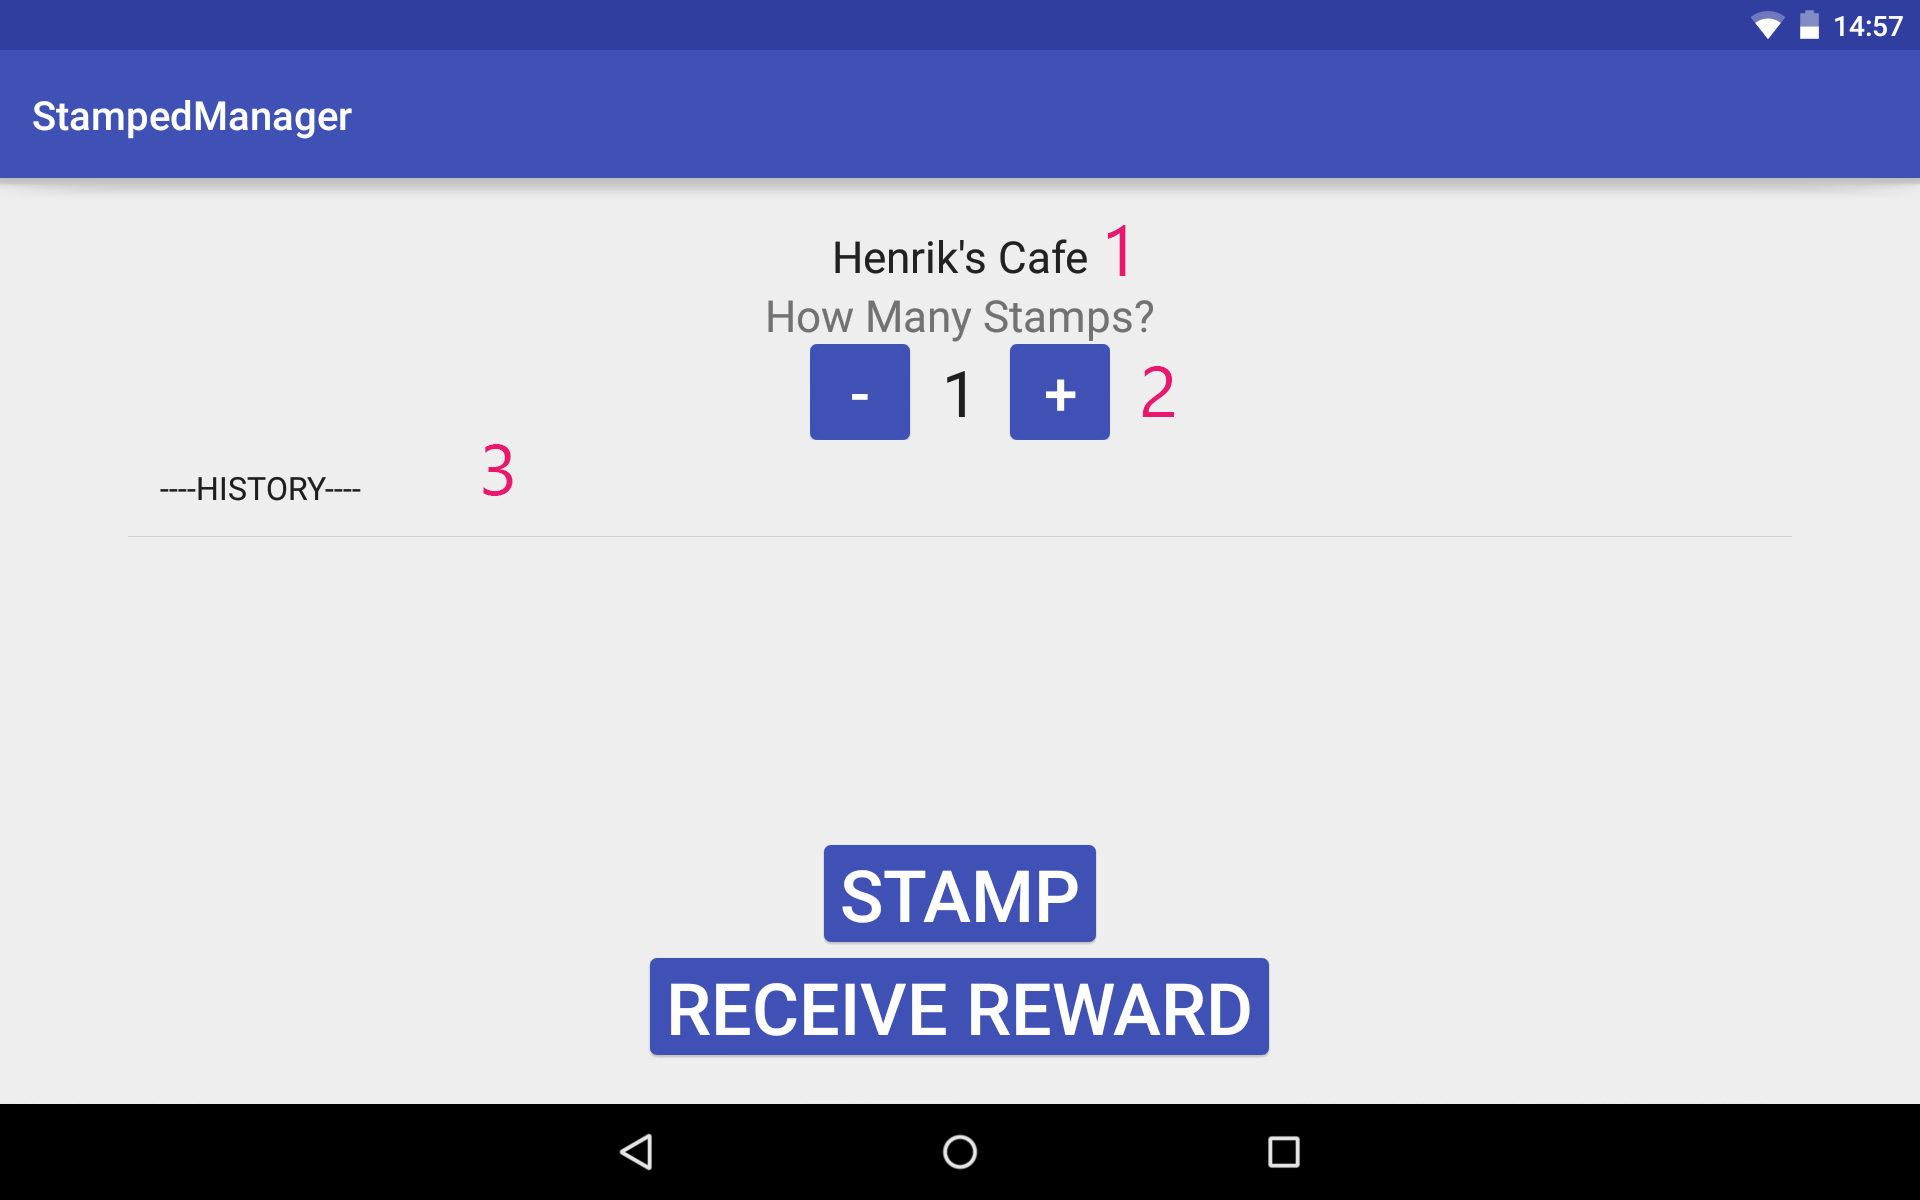
\includegraphics[width=0.494\textwidth]{img/readerfinalmock2.png}
   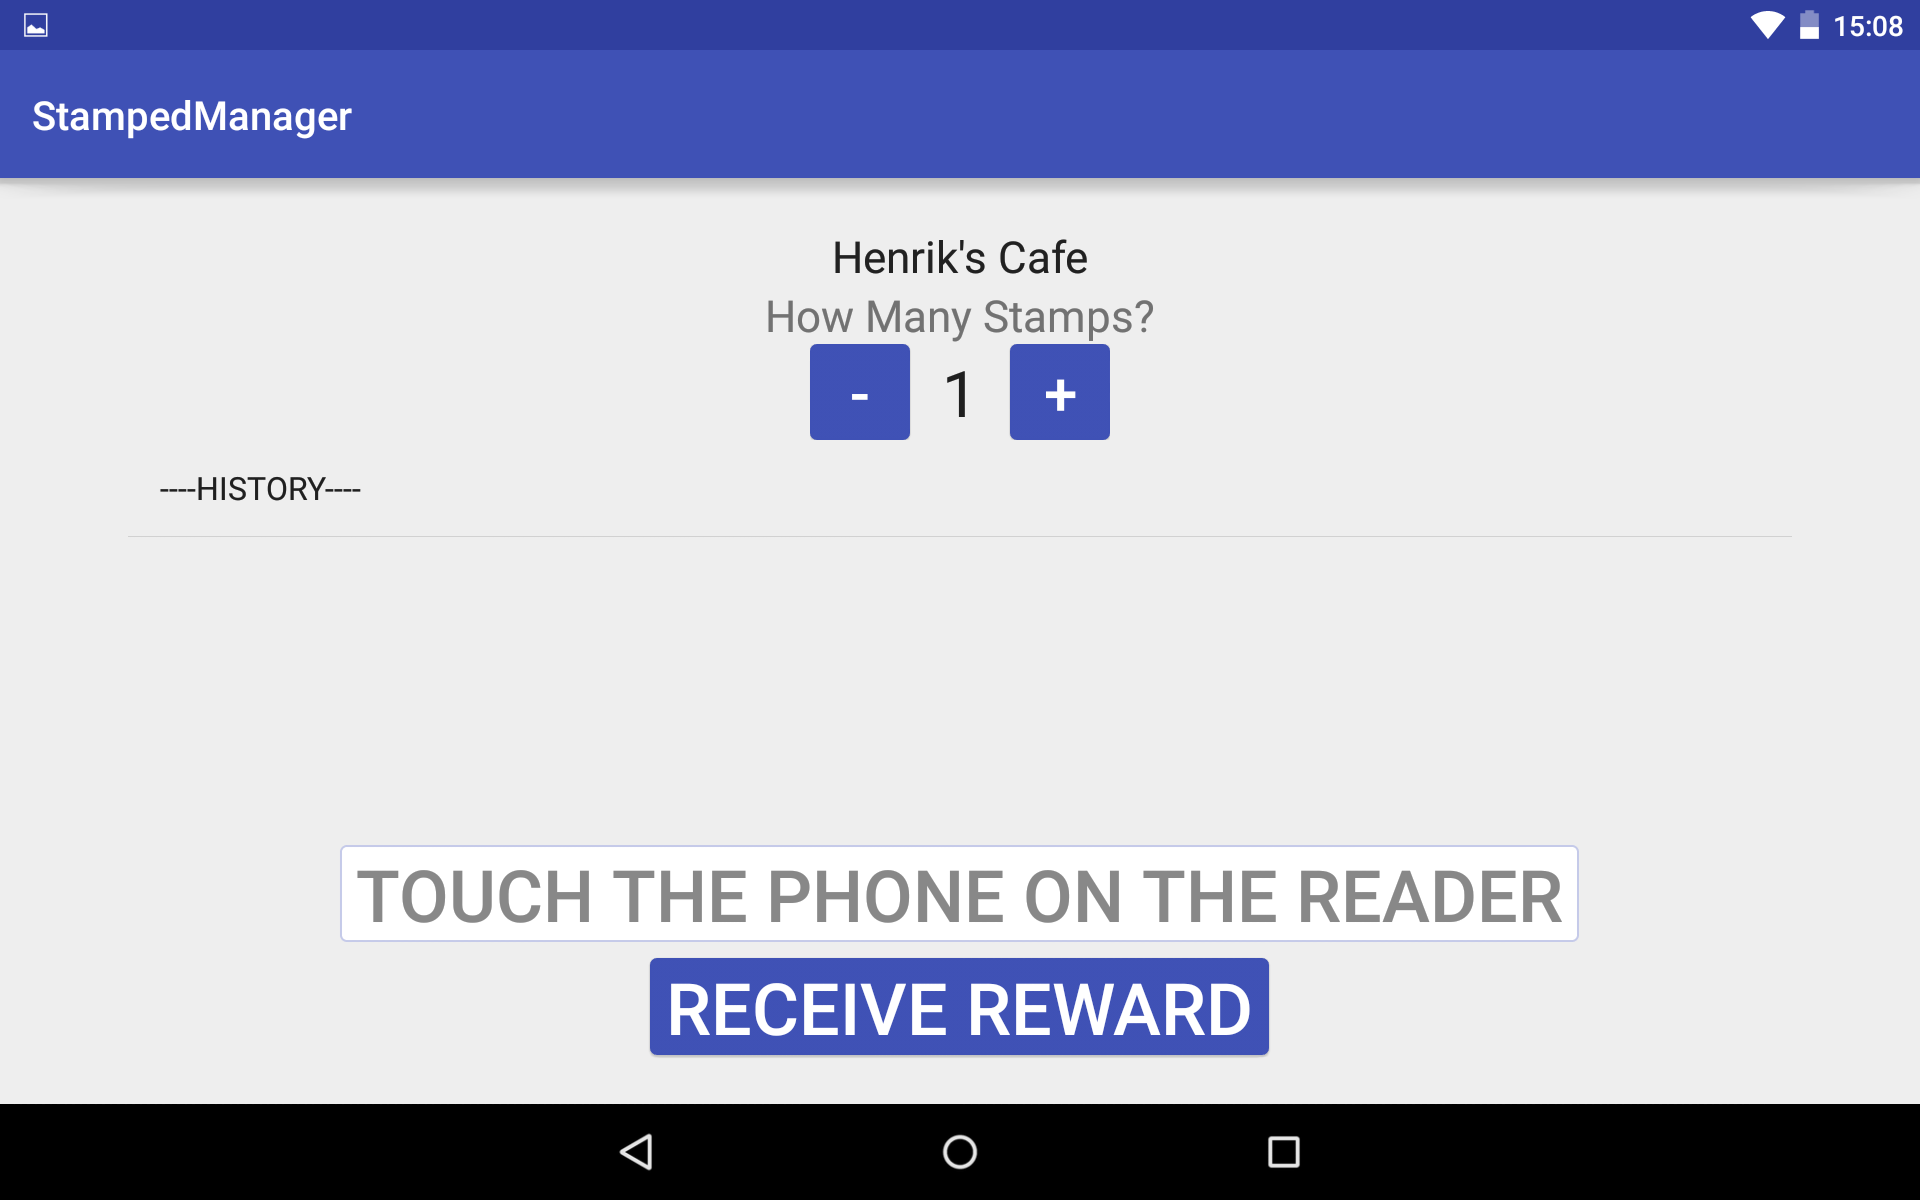
\includegraphics[width=0.494\textwidth]{img/readerfinalmock1.png}
     \caption{The final design of the Stamped Manager with the final aesthetic}
     \label{fig:wireframemr2}
\end{figure}

\subsubsection{Feedback For Next Iteration}
The design was present to three potential users individually, along with all participants during the evaluation. A list of their suggestions follows:
\begin{itemize}
  \item \textit{``The buttons could be bigger like the original design''}
  \item \textit{``There should exist an option to go back to the select a scheme page''}
  \item \textit{``Transaction history need a way to be backed up''}
  %Transaction history PII
\end{itemize}

The feedback for this design mainly came from the employees that tested the system. Bigger buttons seemed to be the primary request. On the other hand, as with the Stamped application, these changes are advised under future work.

\section{Miscellaneous Feedback}
\subsection{Customisability}
Participants expressed a keen interest in  improving the customisability of their profile. Although badges and titles received a positive response, by increasing user customisation, users will be more inclined to spent time in creating their profile; therefore encouraging their investment to the system~\cite{winWithGamification}. Another type of customisation would be to allow users to have more control over their schemes (i.e. arrange them by preference, sort by proximity to businesses, delete unused schemes etc).
\subsection{Invite Friends/Get Rewards}
\label{sec:invite}
One participant recommended the ability to invite friends as a means to get rewards/grow the Stamped ecosystem. In fact, many gamified systems have a social element. There are two possible reasons for this, to be able to show off earned status (leaderboards, badges) to friends and to pander to the viral coefficient~\cite{viral}. The viral coefficient represents the spread of a system/campaign through referrals by current adopters. A high viral coefficient models the growth of a userbase.%viral coefficient////show off
\subsection{Out of Box Experience}
The application was missing substantial instructions on how to operate the system; instead instructions were instead outlined in the brief and instructions to the participants. We discussed in chapter 2 the notion of tools in Fogg's taxonomy~\cite{fogg1998persuasive} as a method of helping users reach specific goals. Many mobile applications have Out-Of-Box-Experiences (OOBEs) (Fig. \ref{fig:OOBE}). These are one-time screens presented to the user when they first install a mobile application,  serving as a tool with the goal of instructing the user on key functionality to get started.
\begin{figure}[H]
 \centering
  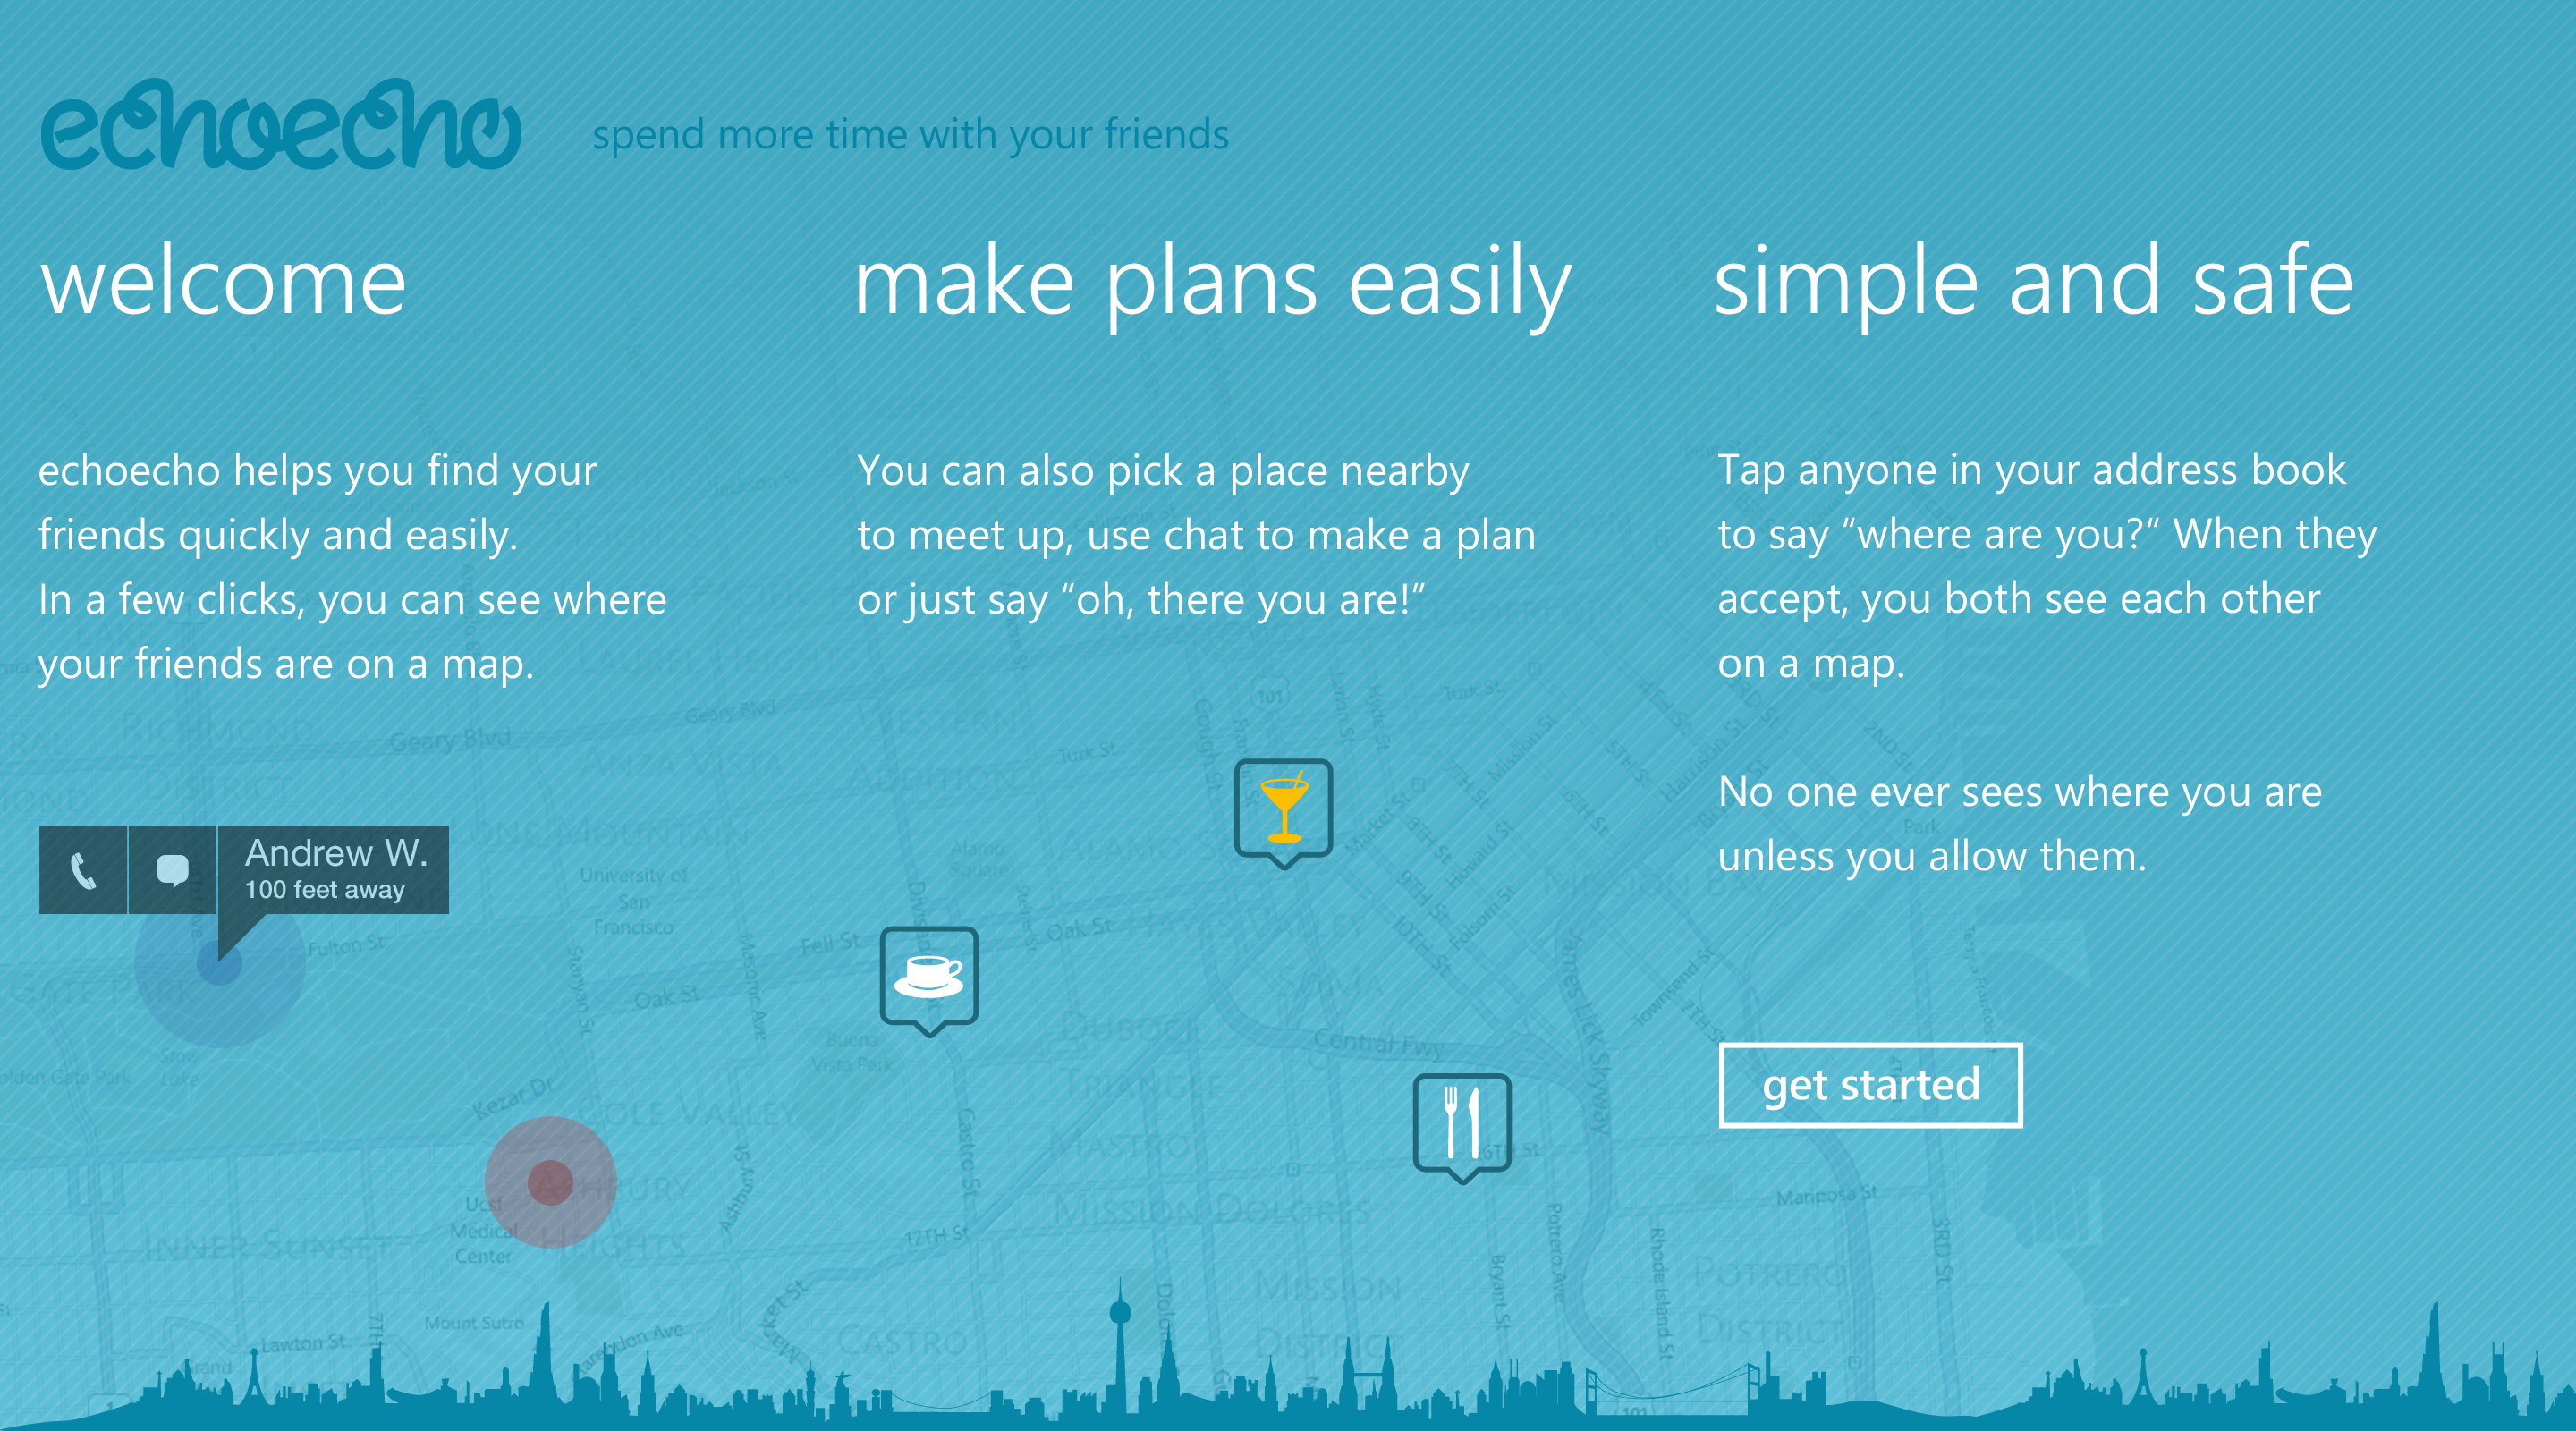
\includegraphics[width=0.6\textwidth]{img/OOBE.png}
     \caption{A panorama of the OOBE found in the \emph{echoecho} application}
     \label{fig:OOBE}
\end{figure}
\section{Conclusion}
In this chapter we looked at the results of our study and the impact gamification has had on the system. We conclude that gamification did indeed bring value to Stamped,

In the next chapter, we summarise our project in terms of its process, contribution to the state of art and ideas for future work.


\chapter{Conclusions \& Future Work}
\section{Conclusions}
Throughout this project, we developed Stamped, a general purpose solution using a smartphone with several advantages over traditional loyalty schemes. We completed our objectives outlined in chapter 1 (listed below).
\begin{itemize}
    \item Research the state-of-art surrounding NFC technology within loyalty and gamification systems
    \item Examine and analyse the current smartphone solutions available to manage loyalty systems
    \item Design and implement our solution
    \item Perform a field study with the system as an evaluation
    \item Look into the future possibilities of the system and the infrastructural requirements to support its use in a real-world environment
\end{itemize}

In our study we identified that gamification, was an enjoyable motivator for our system. Moreover, we showed that users prefer and see the value of the `tapping' method over classical stamp-cards.

With the cost of developing mobile applications going up with the advancement of mobile technologies, the barriers of entry for small businesses can be too difficult. With Stamped, we believe that we have developed a flexible novel way for any business, big or small, to create and deploy a simple loyalty schemes. The generality of the system affords many different types of loyalty schemes --- from gym passesas to bike miles to coffee shops. Although developed on Android, the protocols are generic enough to allow the system to be homogeneous to any mobile operating system or even smart cards.

With Stamped, we believe that we have contributed a system that gives rise to NFC in our modern lives. Even though for a long time, this technology has been seen as a niche, we hope that this inspires a new generation of NFC solutions that solve everyday problems.

\section{Future Work}
Even though the system has met the aims and objectives we outlined, there are many directions we can expand the project with regards to future work.
\newpage
\subsection{Making The System Viable}
The system in its current state requires certain additional features to support adoption, some of these include requirements which have yet to be implemented:
\begin{itemize}
	\item Improving the NFC architecture to avoid the problem `weak interactions'
	\item Encrypting messages between the applications to protect the system from abuse
	\item The ability to manage/customize loyalty-schemes in the Stamped Manager
	\item More options for business to incorporate their brand into their loyalty scheme
\end{itemize}

\subsection{Further Studies}
As well as being able to run a larger study with more participants, it is also of value to study these system modifications
\begin{itemize}
	\item Experimenting with different types of gamification techniques to see which are most effective for our system
	\item Experimenting with suggesting for users (i.e. learning what kinda of loyalty schemes a user frequents)/providing suggestions similar to the way \emph{Amazon} provides suggestions based on user habits
\end{itemize}

\subsection{Extending Stamped}
The functionality of stamped can be extended by the following:
\begin{itemize}
	\item Adding a social element (collecting schemes with friends, sharing rewards)
	\item Allowing for different types of loyalty schemes, not just stamps based
	\item Integrating maps to identify nearby schemes
\end{itemize}

Additionally we can incorporate some of our `Wont Have' requirements we discussed in Chapter 3:
\begin{itemize}
\item The ability to make payments with the system as well as collect stamps
\item Allowing the ability to gift/share rewards with friends (as a metaphor for gift cards)
\end{itemize}
\newpage
The application can also be expanded in the following ways:
\begin{enumerate}
\item Porting to iOS and Windows platforms
\item Deep integration with Electronic Point Of Sales (EPOS) systems
\item Incorporating further smartcard activities using NFC
\item Porting to smartwatches (using NFC found in smartwatches to collect stamps as well as the phone)
\item Adding a health element, tracking a users physical activity and rewarding them accordingly
\item Integrating all of the uses of a company/university smartcard (e.g. access to site, payments) as functionality
\end{enumerate}

We believe that Stamped promotes a novel method of managing a daily inconvenience. As a proof of concept, we outlined many directions several different directions the application can evolve to fit into the lives of the user. Perhaps the system could even be revised to incorporate more card-based services such as ticketing.

We're living in a time where contactless technologies are seeing heavy investment --- from bank cards to interactive toys, users are being exposed to newer and more efficient methods to enrich once tedious tasks. Is it possible that one day we'll live in a world where you can interact with anything with a tap?



%%
%% Now we are back to the standard project contents that you should include
%%
\bibliographystyle{ieeetr}
\bibliography{bib}

\appendix

%%
%% Use the appendix for major chunks of detailed work, such as these. Tailor
%% these to your own requirements
%%

\chapter{Interview Transcript}
\textbf{Tell me quickly about your role}

I am a Business Analyst for the WREF (Worldwide Real Estate and Facilities) IT. My role within IT is facilitating any technological solutions required or requested by the WREF team; on or off-site.

\textbf{What are Bike Miles within COMPANY A}

Bike Miles within COMPANY A is a loyalty scheme for permanent COMPANY A staff members at 3 UK sites. Under the scheme, users who enter those sites are entitled to a sticker, which equates to £1 that can be spent in the bike shop (Evans Cycles). From the 3 sites that have the Bike Miles scheme, there are approximately 7000 staff members with 2100 users registered to the scheme of this, 800 active users (active users are those who have claimed more than £50 within the last year).This scheme is used to encourage our staff to get fit by riding to work, save the environment and help reduce the need for parking with the very limited spaces available at sites.

\textbf{What's the current scenario now}

The current scenario consists of the following:
\begin{enumerate}
\item Users come to the security barrier on site
\item They tear off a sticker
\item They then use their COMPANY A pass which opens the barrier, enabling them to enter the site
\item The sticker is put into a collecting paper card
\item The paper collection card is presented to the bike shop for money off 
\end{enumerate}

\textbf{What problems are there to tackle?}

With the existing there are a lot of problems to tackle as we believe people are abusing the system.
\begin{itemize}
\item Anyone can enter the scheme – Therefore we cannot track who is actually regularly riding their bikes onto sites. In regards to the 800 users listed above, they could potentially come into site in a car and still take a sticker.
\item People are taking more than one sticker at a time, with no security preventing the problem
\item Contractors are not entitled to the scheme, but could still take the stamps.
\item We believe there is a ‘black market’ for the stamps whereby users are taking the stamps and passing/selling them on to other staff members.
\end{itemize}

\textbf{What solutions have you guys thought about}

We have looked at other ideas to try and overcome the problem, but under current COMPANY A policy no new applications can be submitted into the current pool of apps. With that in mind a solution was required whereby staff could use their existing COMPANY A card to enter site and store Bike Money, or something similar with a smartphone:
\begin{itemize}
\item COMPANY As corporate device is the iPhone, an application with a QR code scanner which increments on a daily basis upon entering site
\item NFC solution with sticker on the back of existing staff card – Or with the new iPhone 6 this is already incorporated.
\item Fingerprint scanner (but no new applications)
\end{itemize}

\textbf{What do you think of this solution? ( The corporate loyalty app)}

For this solution to be feasible and useful, it would need to be:
\begin{itemize}
\item Available for all of our permanent staff to use
\item Easy integration for further sites and users globally
\item Good usability aspects. COMPANY A has 100,000 staff members with a variety of demographics, therefore all users should find it easy to use and better than the existing process
\item The system would need to increment on a daily basis when the staff members enter site (once a day only)
\end{itemize}
The corporate loyalty scheme is a great idea. Not only could it combat the issue of Bike Miles, as listed above, but it could also be used in conjunction with a lot of the other internal schemes that we have on site, such as Coffee loyalty scheme, gym membership, COMPANY A product store discounts (including online) etc.

\textbf{Could it be considered by COMPANY A?}

COMPANY A are always looking to improve, therefore if a product is received that significantly improves an existing process / technology it may be considered. Mobile phone applications have become more popular in general in recent years and this has rubbed off on COMPANY A staff members to change their perception (who previously were against mobile technologies). Also off the back of our recent success in winning an award for the Best Use of Mobile Technology Award (COMPANY A SiteMap App) we believe that mobile products can enhance our reputation internally and externally.

\chapter{Initial Wireframes}
\begin{figure}[H]
 \centering
  \includegraphics[width=1\textwidth]{img/Page1.jpg}
     \caption{The initial wireframes for the Stamped system}
\end{figure}
\chapter{Permission Slip}
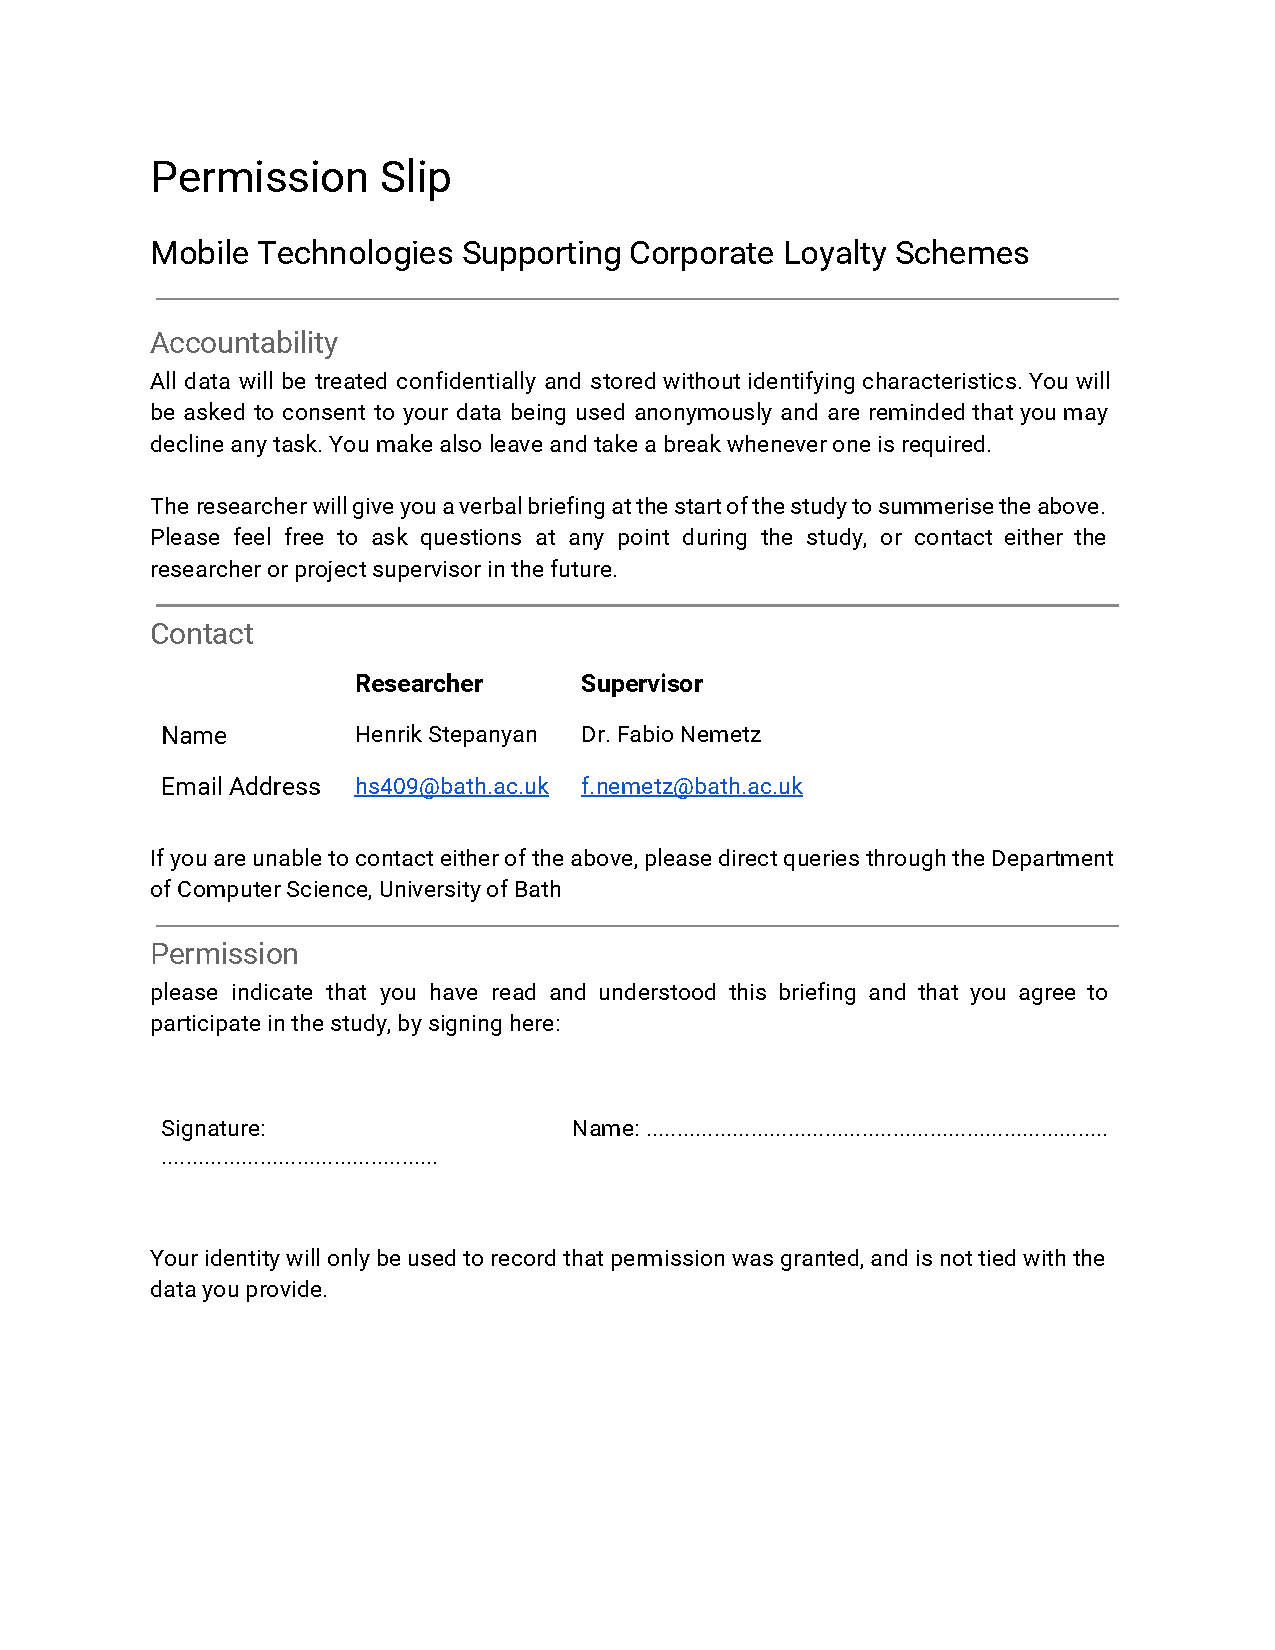
\includepdf[pages={1}]{PermissionSlip.pdf}
\chapter{Briefing Script}
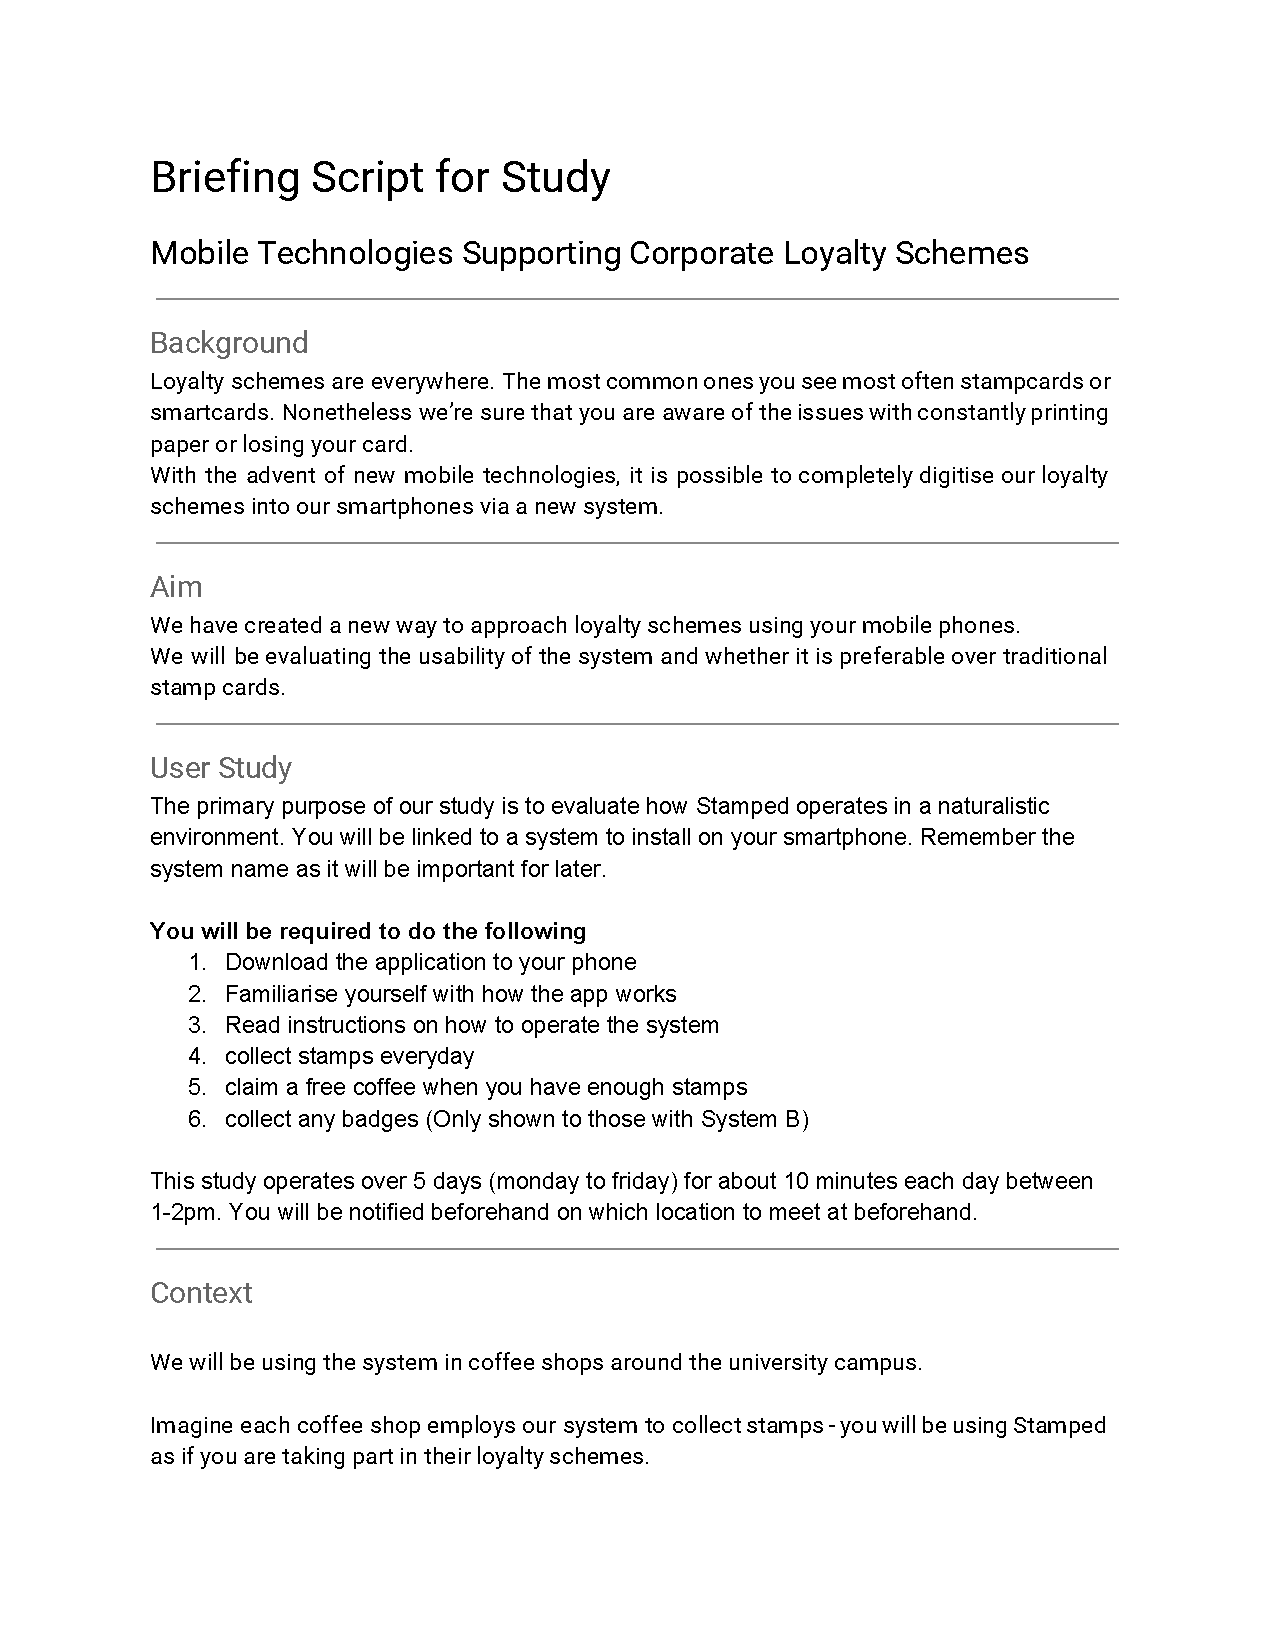
\includepdf[pages={1}]{brief.pdf}
\chapter{Instructions For Study}
\paragraph{Installation Instructions}

\begin{enumerate}
  \item Browse to [link]
  \item Download the application
  \item Go to Settings > Security - Ensure that `Unknown sources' are enabled
  \item Install the downloaded application
  \item login with your university email - the password is 1234
\end{enumerate}

\paragraph{Stamping Instructions --- Stamped}

\begin{enumerate}
  \item Ensure your phone is unlocked (you do not need to have the application open)
  \item Swipe your phone onto the reader when asked
  \item Click on the notification/open the application
  \item Ensure you received a stamp
\end{enumerate}

\paragraph{Claiming a Reward --- Stamped}

\begin{enumerate}
  \item Open the application
  \item Ensure you have 5 stamps in the loyalty scheme `Bath Cafe`
  \item Swipe to the rewards tab
  \item Select the available reward `free coffee`
  \item Notify the employee that you want to claim a reward
  \item Swipe your phone onto the reader when asked
  \item Open the application and ensure your stamps have been deducted
\end{enumerate}

\paragraph{Instructions --- Stamped Manager}

\begin{enumerate}
  \item (for stamping) Use the `+' and `-' buttons in order to select the number of stamps to distribute
  \item press appropriate button for stamping/reward claiming
  \item ask customer to Swipe their phone onto the reader
\end{enumerate}

\chapter{Participant Questionnaire}
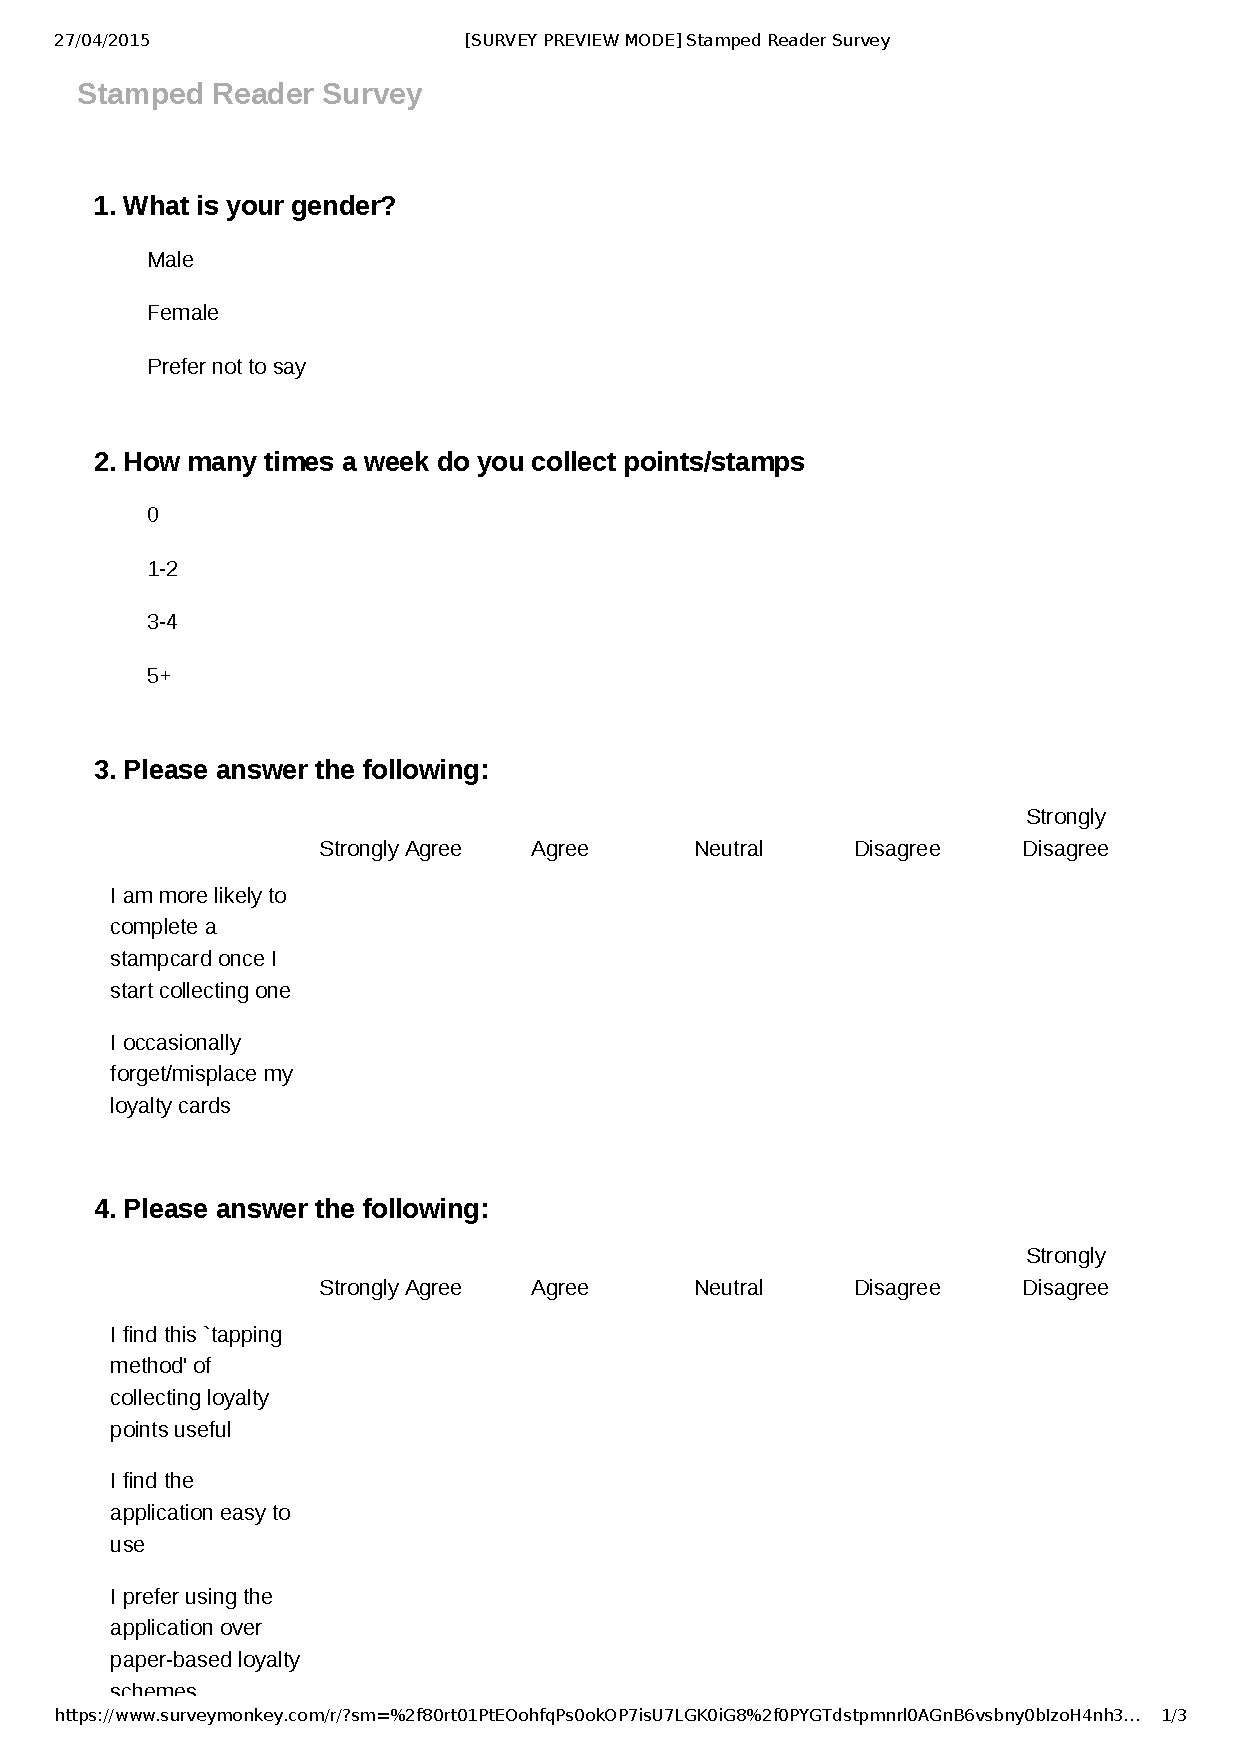
\includepdf[pages={1,2}]{questionnaire1.pdf}
\chapter{Employee Questionnaire}
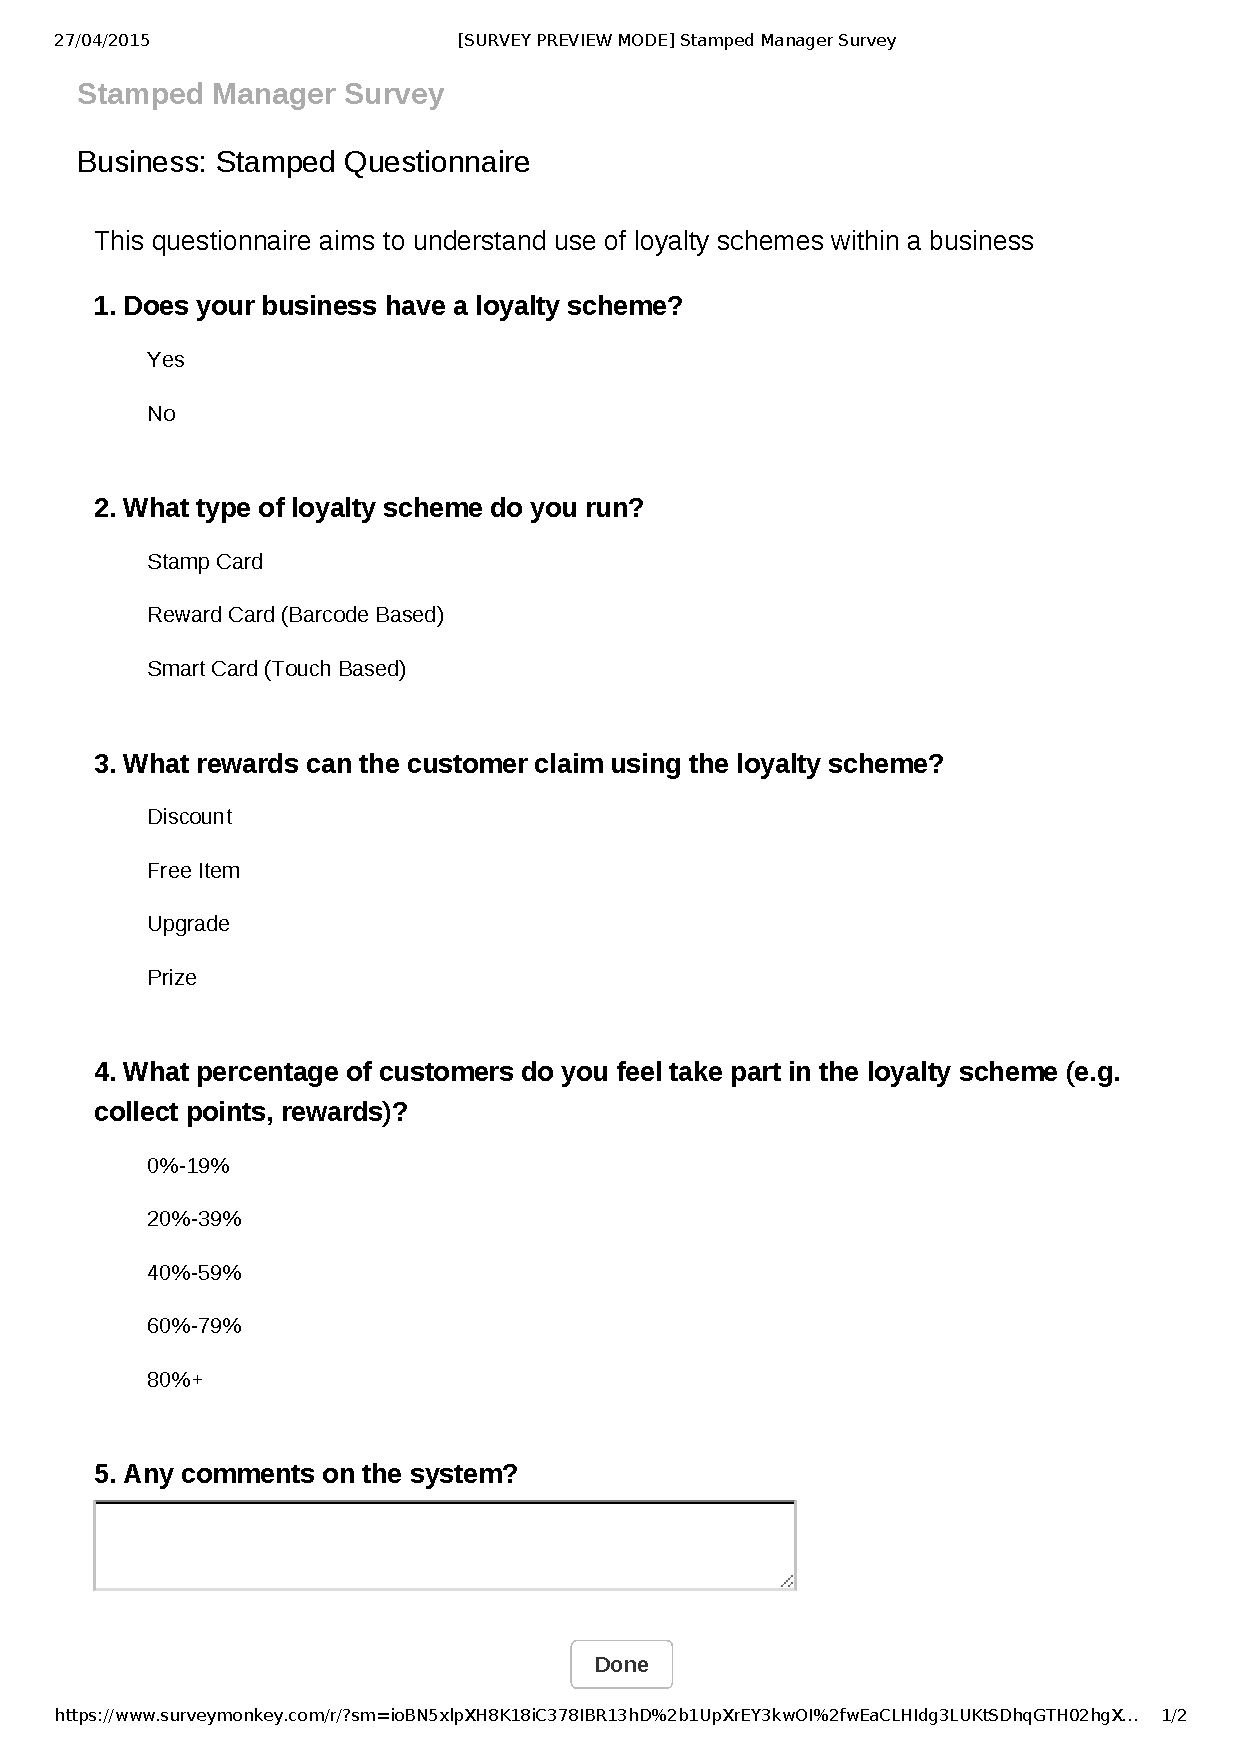
\includepdf[pages={1}]{questionnaire2.pdf}
\end{document}